%% -*- coding:utf-8 -*-
\chapter{Valenz, Argumentabfolge und Adjunktstellung}
\label{chap-valence}

%\if0
Dieses Kapitel behandelt die Repräsentation von Valenzinformation und skizziert die grundlegenden Strukturen, die
für SVO- und SOV-Sprachen angenommen werden. Ich entwickle eine Analyse des Scramblings in denjenigen Sprachen, die
es zulassen, und diskutiere die feste vs.\ freie Stellung von Adjunkten.

\section{Valenzrepräsentationen}
\label{sec-valence}

Die\is{Valenz|(} Wortfolgen in (\mex{1}) wurden bereits in Fußnote~\ref{fn-ex-das-kind-erwartet} auf
Seite~\pageref{fn-ex-das-kind-erwartet} diskutiert.
\eal
\ex[*]{der Delphin erwartet}
\ex[*]{des Kindes der Delphin den Ball dem Kind gibt}
\zl
Das Problem ist, dass zu wenige (\mex{0}a) oder zu viele NPs (\mex{0}b) vorhanden sind. Das Konzept,
das hier benötigt wird, ist die Valenz: Wie in der Chemie wird angenommen, dass Köpfe ein bestimmtes Potential
haben, stabile Verbindungen mit anderem Material einzugehen \citep[\page 239]{Tesniere2015a-u}. Zum Beispiel
verlangt das Verb \emph{erwarten} eine NP im Nominativ und eine im
Akkusativ. \emph{geben} ist das prototypische ditransitive Verb: Es kann mit einer
NP im Nominativ, einer NP im Dativ und einer NP im Akkusativ kombiniert werden, aber wie (\mex{0}b) zeigt, kann ein
Genitivobjekt nicht in einen Satz integriert werden.

Die NPs in den Beispielen in (\mex{1}) sind Argumente der jeweiligen Verben:
\eal
\ex[]{{}[dass] der Delphin den Menschen erwartet}
\ex[]{{}[dass] der Delphin dem Kind den Ball gibt}
\zl
Die meisten syntaktischen Argumente füllen außerdem eine sogenannte \term{semantische Rolle} in der semantischen Repräsentation des
Kopfes aus. Zum Beispiel ist der Delphin der Gebende, das Kind der Empfänger und der Ball das gegebene
Objekt. \citet[Chapter~48]{Tesniere2015a-u} schlug vor, zur Erklärung der Valenz die Analogie zu Dramen zu verwenden: Wenn wir
uns die Szene des Gebens vorstellen, was muss auf der Bühne geschehen, damit ein dargestelltes Ereignis ein Gebe"=Ereignis
genannt werden kann? Es muss die drei Beteiligten geben, einen Gebenden, einen Empfänger und etwas, das
gegeben wird. Ohne diese Beteiligten haben wir kein richtiges Gebe"=Ereignis.

Zusätzlich zu Elementen wie den NPs in den obigen Beispielen, die Argumente\is{Argument} genannt werden,
gibt es auch sogenannte Adjunkte. \emph{schnell} (\mex{1}a) und \emph{quickly} (\mex{1}b)
sind Beispiele für Adjunkte:
\eal
\ex \dass{} der Delphin dem Kind schnell den Ball gibt
\ex that the dolphin gives the child the ball quickly
\zl
Die Adverbiale liefern zusätzliche Information über das Gebe"=Ereignis, aber sie füllen keine
semantische Rolle aus. Während die Form von Argumenten oft durch ihre
Köpfe bestimmt wird, wird die Form von Adjunkten nie durch den Kopf bestimmt, mit dem sie kombiniert werden. Zum Beispiel wird die Wortart
von Subjekten und Objekten, die Argumente sind, durch ihre
Köpfe bestimmt. \emph{unterstützen} nimmt eine NP im Nominativ und eine NP im
Akkusativ (\mex{1}a). Das Verb \emph{helfen}, das semantisch \emph{unterstützen} recht ähnlich ist,
nimmt eine Nominativ-NP und eine Dativ-NP (\mex{1}b). Zweiwertige Verben nehmen üblicherweise ein Akkusativobjekt,
sodass Deutschlernende die Tatsache, dass \emph{helfen} einen
Dativ nimmt, explizit lernen müssen. (\mex{1}c) ist ein Beispiel mit einem Präpositionalobjekt. Das Verb \emph{warten}
verlangt eine PP mit der Präposition \emph{auf} und eine Akkusativ-NP innerhalb der PP.
\eal
\ex Ich unterstütze ihn.
\ex Ich helfe ihm.
\ex Ich warte \emph{auf} \emph{ihn}.
\zl
Die Form von Adjunkten wird nie durch ihre Köpfe bestimmt. NPs, PPs, Adjektive, Adverbien und Sätze können
Adjunkte sein:
\eal
\ex Aicke redet den ganzen Tag.
\ex Aicke redet vor dem Rathaus.
\ex Aicke redet laut.
\ex Aicke redet oft.
\ex Aicke redet, weil Protest nötig ist.
\zl

Um die Sache zu verkomplizieren: Nicht alle Argumente müssen in einem
Satz realisiert werden.\label{page-optional-arguments} Das ditransitive Verb \emph{geben} kann
mit jeder Teilmenge seiner Argumente realisiert werden, sofern der Kontext die fehlende Information ergänzt.
\eal
\ex Sie gibt Geld.
\ex Sie gibt den Armen.
\ex\label{ex-sie-gibt} Sie gibt.
\ex Gib!
\zl
%\largerpage
Im Fall von (\mex{0}a) könnte ein bestimmtes Wohltätigkeitsszenario etabliert worden sein, und man kann entweder
Essen oder Geld spenden oder etwas freiwillige Arbeit beisteuern. In einer solchen Situation ist (\mex{0}a) völlig
in Ordnung. Das übertragene Objekt in (\mex{0}b) ist wahrscheinlich Geld. Ein möglicher Kontext für (\mex{0}c) und
(\mex{0}d) ist das Kartenspiel Skat, bei dem die Person, die gibt, unter den
Spielern wechselt. (\mex{0}d) ist ein Imperativ. Selbst Subjekte können in Imperativen weggelassen werden, da der Referent
des Subjekts offensichtlich ist: Es ist der Adressat der Äußerung.

Die Beispiele in (\mex{0}) zeigen, dass die Argumente von \emph{geben} weggelassen werden können. Dies ist
beim Akkusativobjekt von \emph{erwarten} nicht der Fall: Es ist obligatorisch. Argumente können also
optional oder obligatorisch sein, aber Adjunkte sind immer optional. Abbildung~\ref{fig-optional-arguments-adjuncts}, die
der Duden-Grammatik entnommen ist \citep[§1182]{Duden2005}, veranschaulicht dies.
\begin{figure}
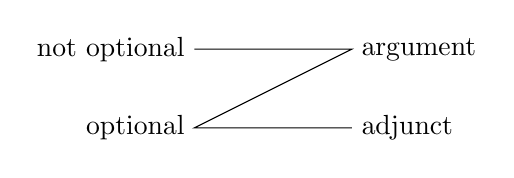
\begin{tikzpicture}
\node[anchor=east](c1) at (-1,2) {not optional};
\node[anchor=east](c2) at (-1,1) {optional};
\node[anchor=west](c3) at (1,2) {argument};
\node[anchor=west](c4) at (1,1) {adjunct};
\draw (c1.east) -- (c3.west) -- (c2.east) -- (c4.west);
\end{tikzpicture}
\caption{\label{fig-optional-arguments-adjuncts}Adjunkte sind immer optional, Argumente können
  optional oder obligatorisch sein \citep[§1182]{Duden2005}}
\end{figure}

Während die Anzahl der Argumente begrenzt ist (durch die Anzahl der verfügbaren Stellen), ist die Anzahl der Adjunkte es nicht: Es kann
beliebig viele Adjunkte in einer Phrase geben. (\mex{1}) zeigt ein Beispiel mit zwei Adjunkten:
\ea
\dass{} der Delphin jetzt dem Kind schnell den Ball gibt
\z

\noindent
Die Analogie mit der Chemie und dem Drama kann verwirrend sein, da H$_2$O ein sehr schönes und stabiles Molekül
ist und es hilfreich ist, sich die parallele Kombination eines Verbs mit seinen beiden
Argumenten vorzustellen. Abbildung~\vref{fig-chemistry-valence} zeigt H$_2$O und die parallele Kombination eines Verbs
mit seinen Argumenten entsprechend (\mex{1}a). Das Problem ist, dass ein einzelnes H und ein O keine
stabile Verbindung bilden, während (\mex{1}b) in Ordnung ist:
\eal
\ex Kirby helps Sandy.
\ex Kirby helps.
\zl
\begin{figure}
\centering
\begin{forest}
[O
  [H] 
  [H] ]
\end{forest}
\hspace{5em}
\begin{forest}
[helps
 [Kirby]
 [Sandy] ]
\end{forest}
\caption{\label{fig-chemistry-valence}Kombination von Wasserstoff und Sauerstoff und die Kombination
eines Verbs mit seinen Argumenten}
\end{figure}%
%\largerpage
Natürlich kann man einfach annehmen, dass es eine Version von \emph{helps} gibt, die eine andere Valenz hat
als die üblicherweise angenommene zweistellige Valenz. Hier bricht die Parallele zusammen, da wir kein
Sauerstoffatom mit nur einer offenen Stelle für das Wasserstoffatom haben. Die Drama-Analogie trägt zur
Verwirrung bei, da das in (\mex{0}b) beschriebene Hilfsereignis natürlich jemanden umfasst, dem geholfen
wird. Die Lösung dieses Problems besteht darin, zwischen syntaktischer und semantischer Valenz zu unterscheiden \citep[Section~3]{Jacobs2003a-u}. Die
Drama-Analogie hilft uns, die semantische Valenz zu finden, die Chemie-Analogie betrifft eher die syntaktische Valenz.

Da Chemie und Drama ihre Probleme haben, können wir auf eine
andere\label{page-shopping-analogy} Analogie zurückgreifen: das Essen. Nehmen wir an, Sie möchten eine Mahlzeit mit Nudeln, Tofu und einer
Tomatensoße zubereiten. Für die Tomatensoße brauchen Sie außerdem ein paar Zwiebeln. Sie setzen alle Zutaten auf eine
Einkaufsliste und gehen in den Laden. Im Laden stellen Sie fest, dass der Tofu ausverkauft ist. Ihre Mahlzeit
funktioniert auch ohne Tofu. Tofu ist optional. Glücklicherweise hat der Laden reichlich Nudeln. Sie können
zwischen den verschiedenen Sorten wählen und die Nudelsorte und Marke auswählen, die Sie bevorzugen. Ein paar Zwiebeln, Tomaten,
und Sie sind fertig. Moment, neben der Kasse liegen diese Gummibärchen. Okay, Sie nehmen auch ein paar davon
mit, obwohl Sie das nicht vorhatten und sie nichts mit Ihrer Mahlzeit und Ihrer Einkaufsliste
zu tun haben. Die Gummibärchen sind die Adjunkte.

Zurück zur Linguistik: Es gibt zwei Wege, sicherzustellen, dass Argumente zusammen mit ihren Köpfen realisiert werden. Der erste
verwendet Techniken, die in Kapitel~\ref{chap-psg-xbar} eingeführt wurden. Wenn man flache Phrasenstrukturregeln
verwendet, kann man sicherstellen, dass bestimmte Argumente zusammen mit bestimmten Köpfen auftreten. Eine
Regel ähnlich der in (\mex{1}) wurde als (\ref{ditrans-schema}) auf Seite~\pageref{ditrans-schema} diskutiert.

\ea
\label{ditrans-schema-two}
\begin{tabular}[t]{@{}l@{ }l@{ }l}
S  & $\to$ & NP[\type{nom}] NP[\type{dat}] NP[\type{acc}] V[\type{ditransitive}]\\
\end{tabular}
\z

\noindent
Solche Schemata wurden in der Generalized Phrase Structure Grammar verwendet \citep*{GKPS85a,Uszkoreit87a}, aber sie wurden
später zugunsten lexikalistischer Modelle aufgegeben, das heißt Modelle, die annehmen, dass Information über die
Argumente eines Kopfes in der lexikalischen Beschreibung des Kopfes statt in Phrasenstrukturregeln
kodiert ist \parencites{Jacobson87b}[Section~5.5]{MuellerGT-Eng1}{MWArgSt}. Gründe für die Aufgabe des phrasalen
Ansatzes der GPSG waren Probleme mit sogenannten Teilvoranstellungen von Verbalphrasen \citep{Nerbonne86a,Johnson86a} und mit der Erfassung von
Interaktionen mit der Morphologie \citep[Section~5.5.1]{MuellerGT-Eng1}.\footnote{%
  Beginnend mit der einflussreichen Arbeit von Adele \citet{Goldberg95a} im Rahmen der Konstruktions"=%
  grammatik\indexcxg{} erlebten die phrasalen Ansätze eine Wiederbelebung \citep{GJ2004a}. Phrasale Ansätze sind weit verbreitet
  und werden auch in anderen Frameworks angenommen
\citep{Haugereid2007a,Haugereid2009a,CJ2005a,Alsina96a,Christie2010a,% resultative constructions as phrasal constructions and
ADT2008a,ADT2013a}.            % argue for a phrasal analysis of the (\ili{Swedish}) caused motion construction.
Die Probleme, die zur Aufgabe der GPSG führten, werden
  in der Literatur ignoriert, und neu eingeführte Probleme werden nicht angemessen behandelt. Siehe
  \cites{Mueller2006d,MuellerPersian,MuellerUnifying,MWArgSt,MWArgStReply,MuellerFCG,MuellerLFGphrasal,MuellerPotentialStructure,MuellerGT-Eng,MuellerCxG}
  für einige Diskussion. Es ist zu beachten, dass es auch lexikalische Varianten der Konstruktions"=%
  grammatik gibt. \citet*{SBK2012a} argumentieren mit der Einführung der \sbcg{} explizit für eine
  lexikalische Sicht und zitieren dabei einige der gerade genannten Quellen. Das Framework, das den in diesem Buch
  skizzierten Vorschlägen zugrunde liegt, ist die Konstruktions-HPSG \citep{Sag97a}.
}

In lexikalischen Ansätzen wird die Valenz eines Kopfes in seinem Lexikoneintrag in Form einer Liste mit Beschreibungen
der Elemente repräsentiert, die zur Valenz des Kopfes gehören. (\mex{1}) gibt einige prototypische Beispiele:
\ea
\label{valence-specifications-German}
\begin{tabular}[t]{@{}l@{~}l@{~}l}
a. & \emph{schläft}:        & \sliste{ NP[\type{nom}] }\\
b. & \emph{kennt}:           & \sliste{ NP[\type{nom}], NP[\type{acc}] }\\
%b. & \emph{unterstützt} `supports':  & \sliste{ NP[\type{nom}], NP[\type{acc}] }\\
c. & \emph{hilft}:           & \sliste{ NP[\type{nom}], NP[\type{dat}] }\\
d. & \emph{gibt}:            & \sliste{ NP[\type{nom}], NP[\type{dat}], NP[\type{acc}] }\\
e. & \emph{wartet}:          & \sliste{ NP[\type{nom}], PP[\type{auf}] }\\
\end{tabular}
\z
Die Elemente in solchen Listen stehen in einer festen Reihenfolge. Die Reihenfolge entspricht der Abfolge der
Elemente im \ili{Englisch}en und der sogenannten unmarkierten Abfolge im \ili{Deutsch}en, das heißt, bei ditransitiven Verben
ist die Abfolge üblicherweise nom, dat, acc (siehe \citew{Hoehle82a} für Anmerkungen zur unmarkierten Abfolge). Diese
feste Abfolge wird verwendet, um die Verknüpfung zwischen Syntax und
Semantik\is{Semantik} herzustellen.\is{linking} Dies wird in Abschnitt~\ref{sec-linking} kurz diskutiert.

Bei einer solchen Valenzrepräsentation für ein Verb wie \emph{kennen} kann man ein Schema annehmen,
das ein Element aus der Valenzliste mit dem jeweiligen Kopf kombiniert und alle ungesättigten
Elemente an das Ergebnis der Kombination weitergibt. Alternativ könnte man eine flache Struktur annehmen, in
der alle Argumente in einem Schritt mit einem Kopf kombiniert werden \parencites[34]{GSag2000a-u}[Section~3]{MuellerOrder}. Ich nehme solche flachen Strukturen nicht an, da
dies die Analyse von Adjunkten (siehe Abschnitt~\ref{sec-adjuncts}) erschweren würde \citep[377--378]{MuellerOrder}.
Der erste Schritt der Analyse von (\mex{1}) ist
in Abbildung~\vref{fig-ihn-kennt} dargestellt.\footnote{%
  Es ist zu beachten, dass dies so klingt, als gäbe es eine Reihenfolge, in der die Dinge kombiniert werden müssen. Dies ist nicht
  der Fall. HPSG-Grammatiken sind Mengen von Beschränkungen, die in beliebiger Reihenfolge angewendet werden können. Es ist nur zu
  Erklärungszwecken, dass Analysen im gesamten Buch von unten nach oben erläutert werden.%
}
\ea
\label{ex-dass-niemand-ihn-kennt}
{}[dass] niemand ihn kennt
\z
\begin{figure}
\centerfit{%
\begin{forest}
sm edges
[{V \sliste{ NP[\type{nom}] } }
  [{NP[\type{acc}]} [ihn] ]
  [{V \sliste{ NP[\type{nom}], NP[\type{acc}] }} [kennt]] ] ]
\end{forest}}
\caption{\label{fig-ihn-kennt}Analyse von \emph{ihn kennt}, die Valenzinformation wird in einer Liste repräsentiert}
\end{figure}
Der Lexikoneintrag für \emph{kennt} hat eine Valenzbeschreibung, die zwei NPs enthält. In einem ersten
Schritt wird \emph{kennt} mit seinem Akkusativobjekt kombiniert. Die resultierende Phrase \emph{ihn kennt}
ist etwas, dessen wichtigste Konstituente ein Verb ist. Daher hat sie V als ihr Kategorie"=%
label. Bestimmte wichtige Eigenschaften linguistischer Objekte werden \emph{Kopfmerkmale}\is{Kopfmerkmal} genannt. Die Wortart
ist eine dieser Eigenschaften. Es wird angenommen, dass alle Kopfmerkmale vom Kopf im Baum
automatisch nach oben weitergegeben werden.

Das Element, das noch nicht mit \emph{kennt} kombiniert wurde, ist die \npnom. Sie ist noch
in der Valenzliste von \emph{ihn kennt} repräsentiert. Abbildung~\vref{fig-niemand-ihn-kennt}
zeigt den nächsten Schritt, bei dem \emph{ihn kennt} mit dem Subjekt \emph{niemand} kombiniert wird.
\begin{figure}
\centerfit{%
\begin{forest}
sm edges
[V \eliste
  [{NP[\type{nom}]} [niemand] ]
  [{V \sliste{ NP[\type{nom}] } }
    [{NP[\type{acc}]} [ihn] ]
    [{V \sliste{ NP[\type{nom}], NP[\type{acc}] }} [kennt]] ] ]
\end{forest}}
\caption{\label{fig-niemand-ihn-kennt}Analyse von (\emph{dass}) \emph{niemand ihn kennt}}
\end{figure}
Das Ergebnis ist ein linguistisches Objekt der Kategorie Verb mit der leeren Liste als Valenzrepräsentation.

Wie in Kürze gezeigt wird, ist das Schema, das Strukturen wie das V \eliste{} und V \sliste{ NP[\type{nom}] } in
Abbildung~\ref{fig-niemand-ihn-kennt} lizenziert, eine abstraktere Version der Regel in (\ref{psg-binaer}) auf Seite~\pageref{psg-binaer}.

% This can be depicted as in
% Figure~\vref{fig-valence-German}, which is an example analysis of (\mex{1}).
% \ea
% \label{ex-dass-niemand-ihn-kennt}
% \gll  {}[dass] niemand ihn kennt\\
%       \spacebr{}that nobody.\NOM{} him.\ACC{} knows\\ 
% \glt `that nobody knows him'
% \z
% \begin{figure}
% \centerfit{%
% \begin{forest}
% sm edges
% [{S \eliste}
%   [{NP[\type{nom}]} [niemand;nobody] ]
%   [{V$'$\sliste{ NP[\type{nom}] } }
%     [{NP[\type{acc}]} [ihn;him] ]
%     [{V \sliste{ NP[\type{nom}], NP[\type{acc}]}} [kennt;knows]] ] ]
% \end{forest}}
% \caption{\label{fig-valence-German}Analysis of (\emph{dass}) \emph{niemand ihn kennt} `that nobody
%   knows him', valence information is represented in a list}
% \end{figure}

% The lexical item for \emph{kennt} `knows' has a valence description containing two NPs. In a first
% step \emph{kennt} is combined with its accusative object. The resulting phrase \emph{ihn kennt} `him
% knows' is something whose most importent constituent is a verb. Therefore it has a V in its category
% label. Since \emph{ihn kennt} is not a sentence but something intermediate, it gets the label
% V$'$.\footnote{%
%   These labels are abbreviations for complex categories. Their internal makeup is given in
%   Table~\ref{tab-abbreviations-v-vbar-s} on p.\,\pageref{tab-abbreviations-v-vbar-s}. The labels are
%   similar to what is known from \xbart, but -- as was already mentioned in the previous chapter --
%   the theory developed here is not following all the tenets of \xbart. For example, simple nouns
%   like \emph{house} are N$'$ and there is no \nnull in the analysis of NPs like \emph{the house}.

%   Section~\ref{sec-intro-spr-comps} explains why the abbreviation for \emph{ihn kennt} `him knows' is V$'$ rather than VP.
% }
%
% The nodes for V$'$ and S are licensed by a schema that combined a head with one element of its
% valence list. The full schema will be given in Chapter~\ref{chap-HPSG-light}, but we will discuss a
% simplified version of it in Section~\ref{sec-intro-schemata}.

Es ist wahrscheinlich hilfreich, zu unserer Analogie vom Einkaufen für eine Mahlzeit zurückzukehren. Nehmen wir an, wir verwenden eine App, um
unsere Einkaufslisten zu organisieren. Für unsere aktuelle Mahlzeit brauchen wir Nudeln und Tomaten. Sie sind in der
App in einer bestimmten Reihenfolge aufgeführt (Tomaten, Nudeln), und es sind kleine Bilder an den Produkten angebracht. Sobald
wir etwas gefunden haben, das zu den Nudeln passt, entfernen wir die Nudeln von der Liste, und die verbleibende Liste
enthält ein Symbol, das uns an die Tomaten erinnert. Sobald wir diese haben, entfernen wir sie von der Liste, und
da nichts mehr auf der Liste steht, bezahlen wir. Linguistische Strukturen sind ähnlich: Wir beginnen
mit einem Verb, das zwei NPs selegiert, kombinieren es mit einer NP und dann mit der zweiten. Das Ergebnis ist
eine vollständige Struktur, etwas mit einer leeren Valenzliste.

Es gibt verschiedene Wege, mit optionalen Argumenten umzugehen. Der einfachste ist, weitere
Lexikoneinträge anzunehmen, die weniger Argumente selegieren. Für das Beispiel in (\ref{ex-sie-gibt}) würde man die Valenz"=%
repräsentation in (\mex{1}a) annehmen, und für Sätze mit \emph{warten} ohne Präpositional"=%
objekt würde man (\mex{1}b) zusätzlich zu den Repräsentationen in (\ref{valence-specifications-German}) annehmen:
\ea
\begin{tabular}[t]{@{}l@{~}l@{~}l}
a. & \emph{gibt}:            & \sliste{ NP[\type{nom}] }\\
b. & \emph{wartet}:          & \sliste{ NP[\type{nom}] }\\
\end{tabular}
\z
\is{Valenz|)}

\section{Scrambling: Die allgemeine Idee}
\label{sec-scrambling}

Wie\is{Scrambling|(}\is{Abfolge|(} wir bereits in der Datendiskussion in Abschnitt~\ref{sec-phenomenon-scrambling} gesehen haben, erlauben manche Sprachen
das Scrambling von Argumenten. Für diese Sprachen kann man annehmen, dass ein Kopf mit jedem seiner
Argumente kombiniert werden kann, nicht notwendigerweise beginnend mit dem letzten, wie es bei der Analyse in Abbildung~\ref{fig-niemand-ihn-kennt} der Fall war.
Abbildung~\vref{fig-scrambling-German} zeigt die Analyse von (\mex{1}).
\ea
{}[dass] ihn niemand kennt
\z
\begin{figure}
\centerfit{%
\begin{forest}
sm edges
[{V \eliste}
   [{NP[\type{acc}]} [ihn] ]
   [{V \sliste{ NP[\type{acc}] } }
      [{NP[\type{nom}]} [niemand] ]
      [{V \sliste{ NP[\type{nom}], NP[\type{acc}] }} [kennt] ] ] ]
\end{forest}}
\caption{\label{fig-scrambling-German}Analyse von (\emph{dass}) \emph{ihn niemand kennt};
  Sprachen, die Scrambling erlauben, gestatten die Sättigung von Argumenten in beliebiger Reihenfolge}
\end{figure}
Statt das Verb zuerst mit dem Akkusativargument (dem Objekt) zu kombinieren, wird es mit dem
Nominativ (dem Subjekt) kombiniert, und der Akkusativ (das Objekt) wird in einem späteren Schritt hinzugefügt.%
\is{Scrambling|(}\is{Abfolge|(}

% only for unstressed pronouns.
%Such an analysis predicts that reorderings of arguments are possible in principle and this is
%independent of the question whether arguments are pronominal or not. However, some authors claim
%that the order of pronouns is rigid \citep[131]{Haider2010a}.

\section{SVO: Sprachen mit fester SV-Abfolge und Valenzmerkmalen}
\label{sec-intro-schemata}
\label{sec-intro-spr-comps}

Der letzte Abschnitt hat gezeigt, wie verbletzte Sätze im \ili{Deutsch}en analysiert werden können. Natürlich ist es
leicht vorstellbar, wie sich dies auf VSO-Sprachen erweitert: Der Kopf ist initial und kombiniert sich zuerst mit dem ersten
Element in der Valenzliste und dann mit allen anderen Elementen. Über SVO-Sprachen wurde bislang jedoch nichts
gesagt. In Sprachen wie dem \ili{Dänisch}en, dem \ili{Englisch}en und so weiter werden alle Objekte
nach dem Verb realisiert, wie in (\mex{1}); nur das Subjekt steht vor dem Verb.
\ea
Kim gave Sandy the book.
\z
Das Verb bildet zusammen mit seinen Objekten in einem bestimmten Sinne eine Einheit: Es kann vorangestellt werden (\mex{1}a). Es kann von
dominierenden Verben selegiert werden (\mex{1}b), es kann koordiniert werden\is{Koordination} (\mex{1}c), und es ist der Ort, an den sich Adjunkte anlagern (\mex{1}d--e).
\eal
\ex John promised to read the book and [read the book], he will.
\ex He will [read the book].
\ex Kim [[sold the car] and [bought a bicycle]].
\ex He often [reads the book].
%\ex He [reads the book] often.
\ex \ldots{} [often [read the book] slowly], he will.
\zl
Dies kann angemessen modelliert werden, indem man zwei Valenzlisten annimmt: eine für die Komplemente\is{Komplement} (\comps{} kurz für \textsc{complements}\isfeat{comps}) und
eine für das Subjekt\is{Subjekt}. Die Liste für das Subjekt wird \textsc{specifier}\is{Spezifikator}-Liste
(\spr) genannt.\isfeat{spr}\footnote{%
  Es gibt verschiedene Versionen der HPSG: \citet[Chapter~3.2]{ps} nahm an, dass alle Argumente eines Kopfes
  in einer Liste repräsentiert werden. Diese Liste wurde \subcatl{} genannt. \citet{Borsley87a} argumentierte, dass man
  mehrere Valenzmerkmale (\subj, \spr und \comps) verwenden sollte, und dies wurde in
  \citew[Chapter~9]{ps2} übernommen: Subjekte von Verben wurden über \subj{} selegiert und Determinatoren über
  \spr. \citet*[Chapter~4.3]{SWB2003a} nehmen an, dass sowohl Subjekte als auch Determinatoren über \spr{} selegiert werden, was
  auch in den hier entwickelten Grammatiken angenommen wird. \citet[Section~3.3]{Sag2012a} präsentiert eine Version der HPSG
  namens Sign-Based Construction Grammar (SBCG), die wie 1987 üblich eine Valenzliste für alle Argumente
  annimmt. Diese Rückkehr zu einem aufgegebenen Ansatz kam ohne jede Argumentation. Daher übernehme ich diese
  Variante der HPSG nicht, sondern halte an der Trennung von Subjekten und anderen Argumenten auf \spr{} und \comps{} fest. Ich
  werde \subj{} nicht als Valenzmerkmal verwenden, aber es wird in der Analyse der Verbalkomplexe
  in Kapitel~\ref{chap-verbal-complex} eingeführt.
} Die Spezifikatorliste spielt sowohl in der Analyse von Sätzen als auch in der Analyse von Nominalphrasen eine Rolle. Nomina
selegieren ihren Determinator über \spr{} und alle ihre anderen Argumente über \comps. Abbildung~\vref{fig-svo}
zeigt die Analyse von Satz (\mex{1}) unter Verwendung der Merkmale \spr{} und \comps.
\ea
Nobody knows him.
\z
\begin{figure}
\centerfit{%
\begin{forest}
sm edges
[{V[\spr \eliste, \comps \eliste]}, name=S
   [{NP[\type{nom}]} [nobody] ]
   [V\feattab{
      \spr \sliste{ NP[\type{nom}] }, \comps \sliste{}}, name=VP
     [V\feattab{
         \spr \sliste{ NP[\type{nom}] },\\
         \comps \sliste{ NP[\type{acc}] }} [knows] ]
        [{NP[\type{acc}]} [him] ] ] ]
\node [right=4cm] at (S)
    {
        = S
    };
\node [right=4cm] at (VP)
    {
        = VP
    };
\end{forest}}
\caption{\label{fig-svo}Analyse der SVO-Abfolge mit zwei getrennten Valenzmerkmalen}
\end{figure}
Die \compsl{} von \emph{knows} enthält eine Beschreibung des Akkusativobjekts, und der Akkusativ
\emph{him} wird in einem ersten Schritt mit \emph{knows} kombiniert. Zusätzlich zum Akkusativobjekt
selegiert \emph{knows} ein Subjekt. Diese Selektion wird an den Mutterknoten, die VP, weitergegeben. Daher ist
der \sprv{} von \emph{knows him} identisch mit dem \sprv{} von \emph{knows}. Die VP \emph{knows him}
selegiert eine Nominativ-NP. Diese NP ist in Abbildung~\ref{fig-svo} als \emph{nobody} realisiert. Das
Ergebnis der Kombination von \emph{knows him} mit \emph{nobody} ist \emph{nobody knows him}, was
vollständig ist: Es hat sowohl eine leere \sprl{} als auch eine leere \compsl. Die beiden Regeln, die für
die Kombinationen in Abbildung~\ref{fig-svo} verantwortlich sind, heißen Spezifikator-Kopf-Schema und
Kopf-Komplement-Schema. Ich verwende VP als Abkürzung für etwas mit verbalem Kopf und einer leeren \compsl{} und mindestens
einem Element in der \sprl, und S als Abkürzung für etwas mit verbalem Kopf und leeren Listen sowohl
für \spr{} als auch \compsv.

In Abschnitt~\ref{sec-scrambling} wurde erklärt, wie Scrambling erfasst werden kann: Die Regeln, die
Köpfe mit ihren Argumenten kombinieren, können die Argumente in beliebiger Reihenfolge von der Liste nehmen. Für Sprachen
mit strengeren Anforderungen an die Konstituentenabfolge sind die Regeln strenger: Die Argumente müssen
konsequent vom Anfang oder vom Ende der Liste genommen werden. So beginnt man für das \ili{Englisch}e und das \ili{Dänisch}e
am Anfang der Liste, und für kopffinale Sprachen ohne Scrambling beginnt man am Ende
der Liste. Abbildung~\ref{fig-svo-ditrans} zeigt die Analyse eines Satzes mit einem ditransitiven Verb.
\begin{figure}
\centerfit{%
\begin{forest}
sm edges
[{V[\spr \eliste, \comps \eliste]}
   [{NP[\type{nom}]} [Kim] ]
   [V\feattab{
      \spr \sliste{ NP[\type{nom}] }, \comps \sliste{}}
     [V\feattab{
         \spr \sliste{ NP[\type{nom}] },\\
         \comps \sliste{ PP[\type{to}] }}
       [V\feattab{
           \spr \sliste{ NP[\type{nom}] },\\
           \comps \sliste{ NP[\type{acc}], PP[\type{to}] }} [gave] ]
         [{NP[\type{acc}]} [a book, roof] ] ]
       [{PP[\type{to}]} [to Sandy, roof] ] ] ]
\end{forest}}
\caption{\label{fig-svo-ditrans}Analyse der SVO-Abfolge mit zwei getrennten Valenzmerkmalen und zwei
  Elementen in \comps}
\end{figure}
Das Akkusativobjekt ist das erste Element in der \compsl{} und wird zuerst mit dem Verb
kombiniert. Das Ergebnis der Kombination ist eine verbale Projektion, die die PP[\type{to}] als einziges
Element in der \compsl{} hat. Sie wird im nächsten Schritt mit einer passenden PP kombiniert, was zu einer verbalen
Projektion mit einer leeren \compsl{} (einer VP) führt.

Die Analyse unseres ersten \ili{Deutsch}en Beispiels in Abbildung~\ref{fig-niemand-ihn-kennt} verwendete keinen Namen
für die Valenzliste. Die Frage ist also: Wie verhält sich die Analyse des \ili{Deutsch}en zur Analyse des
\ili{Englisch}en mit \spr{} und \comps? Viele Forscher aus verschiedenen Frameworks haben argumentiert, dass es nicht
sinnvoll ist, in Grammatiken des \ili{Deutsch}en die Subjekte finiter Verben von anderen Argumenten zu unterscheiden. Alle Tests, die
verwendet wurden, um zu zeigen, dass sich Subjekte im \ili{Englisch}en von Komplementen unterscheiden, gelten nicht für die Argumente
finiter Verben im \ili{Deutsch}en. Zum Beispiel wird argumentiert, dass Subjekte -- im Gegensatz zu Objekten --
Extraktionsinseln sind\is{Insel} \parencites[\page 249--250]{Chomsky73a}[\page 76]{Fanselow87a}[\page 35--36]{Grewendorf89a}, das heißt, nichts kann
aus einem Subjekt vorangestellt werden. Aber \citet[\page 173]{Haider93a} zeigt anhand der Beispiele in (\mex{1}), dass dies für das
\ili{Deutsch}e nicht gilt.
% Haider2010: 23 allgemein für OV/VO
% Haider 2010: 40 zitiert Haider83 und Haider89
\eal
\ex {}[Über Strauß]$_i$ hat [ein Witz \_$_i$] die Runde gemacht.
\ex {}[Zu drastischeren Maßnahmen]$_i$ hat ihm [der Mut \_$_i$] gefehlt.
\ex {}[Zu diesem Problem]$_i$ haben uns noch [einige Briefe \_$_i$] erreicht.\footnote{\citew[\page 79]{Oppenrieder91a}
}

\zl

%\enlargethispage{3pt}
\noindent
Das \_$_i$ zeigt die Stelle an, an die das vorangestellte Element, das Element im \vf, gehört. Es befindet sich in
allen drei Beispielen innerhalb der Subjekt-NP. Da es im \ili{Deutsch}en keine Subjekt-Objekt-Asymmetrien gibt,
haben Forscher wie \citet[\page 295]{Pollard90a}, \citet[Section~6.3.2]{Haider93a}, \citet[\page
376]{Eisenberg94b} und \citet[\page 57, 78]{Kiss95a} für sogenannte „Subjekt-als-Komplement``-Analysen argumentiert.
Abbildung~\vref{fig-spr-german} zeigt die angepasste Analyse von
(\ref{ex-dass-niemand-ihn-kennt}) -- hier wiederholt als
(\ref{ex-dass-niemand-ihn-kennt-two}):
\ea
\label{ex-dass-niemand-ihn-kennt-two}
{}[dass] niemand ihn kennt
\z
\begin{figure}
\centerfit{%
\begin{forest}
sm edges
[{V[\spr \eliste, \comps \eliste]}, name=S
        [{NP[\type{nom}]} [niemand] ]
        [{V\feattab{
              \spr \eliste, \comps \sliste{ NP[\type{nom}] } }}, name = Vs
          [{NP[\type{acc}]} [ihn] ]
          [V\feattab{
              \spr \eliste,\\
              \comps \sliste{ NP[\type{nom}], NP[\type{acc}]}} [kennt] ]
] ]
\node [right=4cm] at (S)
    {
        = S
    };
\node [right=4cm] at (Vs)
    {
        = V$'$
    };
\end{forest}}
\caption{\label{fig-spr-german}Die Analyse eines deutschen Satzes mit \spr{} und \compsl}
\end{figure}
%\largerpage
Der Unterschied zwischen dem \ili{Deutsch}en und dem \ili{Englisch}en besteht darin, dass das \ili{Deutsch}e alle Argumente in der \compsl{} des
finiten Verbs enthält und keine Argumente in der \sprl. Da die Elemente in der \compsl{} in beliebiger Reihenfolge mit
dem Kopf kombiniert werden können, ist erklärt, warum alle Permutationen von Argumenten
möglich sind. Spezifikatoren werden links von ihrem Kopf realisiert. Dies ist im \ili{Deutsch}en und
\ili{Englisch}en gleich. Für das \ili{Deutsch}e ist dies im verbalen Bereich nicht relevant, aber das Spezifikator-Kopf-Schema, das
in Kürze eingeführt wird, wird in der Analyse von Nominalphrasen verwendet.

Im weiteren Verlauf dieses Buches verwende ich die Abkürzungen in Tabelle~\vref{tab-abbreviations-v-vbar-s}.
\begin{table}
 \begin{tabular}[t]{@{}l@{ = }l}\lsptoprule
             S  & V[\spr \eliste, \comps \eliste]\\
             VP & V[\spr \sliste{ NP[\type{nom}] }, \comps \sliste{}]\\
             V$'$ & alle anderen V-Projektionen außer Verbalkomplexen\\[2pt]
             NP & N[\spr \eliste, \comps \eliste]\\
             N$'$ & N[\spr \sliste{ Det }, \comps \sliste{}]\\\lspbottomrule
             \end{tabular}
\caption{\label{tab-abbreviations-v-vbar-s}Abkürzungen für S, VP und V$'$ sowie NP, N$'$}
\end{table}

\section{Schemata der unmittelbaren Dominanz}

In Abschnitt~\ref{sec-valence} habe ich bereits erwähnt, dass die Nichtterminalknoten in einem Baum, das heißt die
Knoten, die nicht die Blätter des Baumes sind, durch Schemata lizenziert werden, die denen ähneln, die in
Kapitel~\ref{sec-PSG-Merkmale} und~\ref{sec-xbar} eingeführt wurden. Tatsächlich sind die Schemata sogar abstrakter als
\xbar-Schemata, da sie keine Aussagen über die lineare Abfolge der Töchter machen. Die
beiden in diesem Abschnitt diskutierten Schemata sind hier als (\mex{1}) skizziert:
\ea\label{schema-head-spr-and-head-comps-preliminary}
Spezifikator-Kopf\is{schema!Specifier-Head}-Schema und Kopf-Komplement\is{schema!Head-Complement}-Schema (vorläufig)
\begin{tabular}[t]{@{}l@{ }l@{}}
H[\spr \ibox{1}]   & $\to$ H[\spr \ibox{1} $\oplus$ \sliste{ \ibox{2} }, \comps \eliste]\hspace{1em}\ibox{2}  \\
H[\comps \ibox{1}] & $\to$ H[\comps \sliste{ \ibox{2} } $\oplus$ \ibox{1}]\hspace{1em}\ibox{2} \\
\end{tabular}
\z

\noindent
Syntaktische Regeln, wie sie hier verwendet werden, werden üblicherweise Schemata genannt, da sie recht abstrakt sind: Sie
nennen keine spezifischen Kategorien, sondern identifizieren stattdessen bestimmte Information in den Mutter- und Tochterbeschreibungen.
%The details about such schemata will be given in Chapter~\ref{chap-HPSG-light},
Die Details zu solchen Schemata werden in formalerer HPSG-Literatur wie
\citew[Chapter~4]{MuellerLehrbuch3} oder \citew{Abeille:Borsley2021a} angegeben,
aber Abbildung~\vref{fig-spr-head} und
Abbildung~\vref{fig-head-comp} liefern die jeweiligen Baumdarstellungen.
\begin{figure}
\begin{forest}
[H\feattab{\spr \ibox{1}}%,\\
           %\comps \eliste}
  [\ibox{2}]
  [H\feattab{\spr \ibox{1} $\oplus$ \sliste{ \ibox{2} },\\
             \comps \eliste}
  ]]
\end{forest}
\caption{\label{fig-spr-head}Skizze des Spezifikator-Kopf\is{schema!Specifier-Head}-Schemas (vorläufig)}
\end{figure}
Das H steht für \emph{head} (Kopf). Der Begriff \term{Kopftochter} wird für die Tochter verwendet, die entweder
der Kopf einer Phrase ist oder den Kopf der Phrase enthält (\zb das Verb in einem Satz oder das Nomen in einer
Nominalphrase). \emph{append} ($\oplus$) ist eine Relation, die zwei
Listen verkettet. Zum Beispiel ist die Verkettung von \sliste{ \normalfont a } und \sliste{ \normalfont b }
\sliste{ \normalfont a, b }. Die Verkettung der leeren Liste \eliste{} mit einer anderen Liste ergibt
die letztere Liste. Um einige Beispiele zu geben, die in diesem Kapitel relevant sind, betrachte man die Liste
\sliste{ NP[\type{nom}], NP[\type{dat}], NP[\type{acc} ] }. \emph{append} kann verwendet werden, um zwei
Listen aneinanderzuhängen, was unsere Liste auf die folgenden Weisen ergibt:
\eal
\ex \eliste{} $\oplus$ \sliste{ NP[\type{nom}], NP[\type{dat}], NP[\type{acc}] } = \sliste{ NP[\type{nom}], NP[\type{dat}], NP[\type{acc}] }
\ex \sliste{ NP[\type{nom}] } $\oplus$ \sliste{ NP[\type{dat}], NP[\type{acc}] } = \sliste{ NP[\type{nom}], NP[\type{dat}], NP[\type{acc}] }
\ex \sliste{ NP[\type{nom}], NP[\type{dat}] } $\oplus$ \sliste{ NP[\type{acc}] } = \sliste{ NP[\type{nom}], NP[\type{dat}], NP[\type{acc}] }
\ex \sliste{ NP[\type{nom}], NP[\type{dat}], NP[\type{acc}] } $\oplus$ \eliste{} = \sliste{ NP[\type{nom}], NP[\type{dat}], NP[\type{acc}] }
\zl
Das Schema in Abbildung~\ref{fig-spr-head} zerlegt eine Liste so, dass eine Liste mit einem
einzelnen Element ( \sliste{ \ibox{2} } ) und eine Restliste \iboxb{1} entstehen. Nimmt man die
dreielementige Liste mit nom-, dat- und acc-Elementen an, so wäre dies in (\mex{0}c) der Fall, und \ibox{2} wäre NP[\type{acc}] und
\ibox{1} wäre \sliste{ NP[\type{nom}], NP[\type{dat}] }. In diesem Buch hat die \sprl{} höchstens ein Element.\footnote{
  Siehe aber \citew{MOe2013b} für eine Analyse des \isi{object shift}s im \ili{Dänisch}en, die mehrere Elemente in
  der \sprl{} annimmt.
} Es kann eine NP[\type{nom}] im Falle von Verben in den SVO-Sprachen sein oder der Determinator, wenn
der Kopf ein Nomen ist. Wenn man eine Liste mit einem einzelnen Element in eine Liste mit einem Element
und einen Rest aufspaltet, ist der Rest immer die leere Liste. Daher ist \ibox{1} bei den Listen auf der rechten Seite der Gleichungen in (\mex{1}) die
leere Liste, und \ibox{2} ist NP[\type{nom}] bzw.\ Det.
\eal
\ex \eliste{} $\oplus$ \sliste{ NP[\type{nom}] } = \sliste{ NP[\type{nom}] }
\ex \eliste{} $\oplus$ \sliste{ Det } = \sliste{ Det }
\zl

\noindent
Damit ein Schema wie das in Abbildung~\ref{fig-spr-head} anwendbar ist, müssen die Beschreibungen der
Töchter mit den tatsächlichen Töchtern übereinstimmen. Zum Beispiel ist \emph{sleeps} mit der
rechten Tochter kompatibel: Es hat eine NP[\type{nom}] in seiner \sprl. Wenn \emph{sleeps} als
Tochter des Schemas in Abbildung~\ref{fig-spr-head} realisiert wird, wird \ibox{2} als
NP[\type{nom}] instantiiert. Daher muss die linke Tochter mit einer NP[\type{nom}] kompatibel sein. Sie kann
als einfaches Pronomen wie \emph{she} oder als komplexe NP wie \emph{the brown squirrel} realisiert werden. Zwei
Analysen sind in Abbildung~\ref{fig-she-sleeps-the-brown-squirrel-sleeps} dargestellt.
\begin{figure}
\hfill
\begin{forest}
sm edges
[V\feattab{\spr \eliste,\\
           \comps \eliste}
  [{\ibox{1} NP[\type{nom}]} [she]]
  [V\feattab{\spr \sliste{ \ibox{1} NP[\type{nom}] },\\
             \comps \eliste} [sleeps]]]
\end{forest}
\hfill
\begin{forest}
sm edges
[V\feattab{\spr \eliste,\\
           \comps \eliste}
  [{\ibox{1} NP[\type{nom}]} [the brown squirrel,roof]]
  [V\feattab{\spr \sliste{ \ibox{1} NP[\type{nom}] },\\
             \comps \eliste} [sleeps]]]
\end{forest}\hfill\mbox{}
\caption{Kopf-Spezifikator-Phrasen mit einem Subjekt und einem intransitiven Verb}\label{fig-she-sleeps-the-brown-squirrel-sleeps}
\end{figure}
Das \ibox{1} in Abbildung~\ref{fig-she-sleeps-the-brown-squirrel-sleeps} besagt, dass das, was in der
\sprl{} steht, mit dem identifiziert wird, was das andere Element im Baum ist. Ich habe \npnom{} sowohl im NP-Knoten als auch innerhalb der \sprl{} hinter
das \ibox{1} geschrieben, aber es hätte gereicht, \npnom{}
an einer der beiden Stellen zu erwähnen. Die tatsächliche Zahl in der Box spielt keine Rolle. Worauf es ankommt, ist, wo dieselbe
Zahl in den Bäumen oder Strukturen erscheint. Ich beginne üblicherweise mit \ibox{1} an der Spitze des Baumes und
verwende fortlaufende Zahlen für die folgenden Identifikationen.

Abbildung~\ref{fig-nobody-gave-the-child-a-book} auf S.\,\pageref{fig-nobody-gave-the-child-a-book}
unten zeigt eine Beispielanalyse mit einem ditransitiven Verb, an der ebenfalls das Spezifikator-Kopf-Schema
beteiligt ist. Die Spezifikation des \compsv{} der Kopftochter im Spezifikator-Kopf-Schema stellt sicher,
dass das Verb mit seinen Komplementen kombiniert wird, bevor der Spezifikator hinzugefügt wird.

Neben seiner Verwendung für die Analyse von Subjekt"=VP-Kombinationen in den SVO-Sprachen wird das Spezifikator-Kopf-Schema auch
für die Analyse von NPs in allen \ili{germanisch}en Sprachen verwendet. Abbildung~\ref{fig-spr-head-the-squirrel} zeigt die Analyse der NP \emph{the squirrel}.
\begin{figure}
\begin{forest}
[{N[\spr \eliste, \comps \eliste]}
  [\ibox{1} Det [the]]
  [{N[\spr \sliste{ \ibox{1} }, \comps \eliste]} [squirrel]]]
\end{forest}
\caption{\label{fig-spr-head-the-squirrel}Analyse der NP \emph{the squirrel}}
\end{figure}
\emph{squirrel} selegiert einen Determinator, und das Ergebnis der Kombination von \emph{squirrel} mit einem Determinator ist eine
vollständige nominale Projektion, das heißt eine NP. Es gibt auch Nomina wie \emph{picture}, die zusätzlich zu einem
Determinator ein Komplement nehmen:
\ea
a picture of Kim
\z
Die Kombination von \emph{picture} und seinem Komplement \emph{of Kim} ist parallel zur Kombination
eines Verbs mit seinem Objekt in VO-Sprachen mit fester Konstituentenabfolge. Für solche Kombinationen brauchen wir ein eigenes Schema: das Kopf-Komplement-Schema,
das in Abbildung~\ref{fig-head-comp} angegeben ist.
\begin{figure}
\begin{forest}
[{H[\comps \ibox{1}]}
  [{H[\comps  \sliste{ \ibox{2} } $\oplus$ \ibox{1}  ]}]
  [\ibox{2}]]
\end{forest}
\caption{\label{fig-head-comp}Skizze des Kopf-Komplement\is{schema!Head-Complement}-Schemas (vorläufig)}
\end{figure}
%\largerpage
Das Schema spaltet die \compsl{} eines Kopfes in eine Anfangsliste mit einem Element \iboxb{2} auf, das
als Komplementtochter rechts realisiert wird.\footnote{%
  Im Prinzip sind Töchter in der HPSG ungeordnet, so wie sie es in der GPSG waren \citep{GKPS85a}. Spezielle Linearisierungsregeln werden
  verwendet, um einen Kopf relativ zu seinen Geschwistern in einem lokalen Baum zu ordnen. Ein Schema, das einen Baum
  wie den in Abbildung~\ref{fig-head-comp} lizenziert, würde also auch einen Baum mit den Töchtern in einer
  anderen Reihenfolge lizenzieren, sofern man keine Linearisierungsregeln hätte, die dies ausschließen. Siehe
  \citew{MuellerOrder} für einen Überblick über Ansätze zur Konstituentenabfolge in der HPSG. Lineare Präzedenz"=%
  regeln werden in Abschnitt~\ref{sec-lp-rules} ausführlicher diskutiert.
}
Dieses Schema lizenziert sowohl die Kombination von \emph{gave} und \emph{the child} als auch die Kombination von
\emph{gave the child} und \emph{a book} in Abbildung~\vref{fig-nobody-gave-the-child-a-book}, die die
Analyse von (\mex{1}) zeigt.\footnote{%
  \ili{Englisch}e Nomina und Determinatoren flektieren nicht nach Kasus. Der Kasus zeigt sich jedoch in Pronomina:
  \emph{he} (Nominativ), \emph{his} (Genitiv), \emph{him} (Akkusativ). Daher selegieren Verben in Doppelobjekt"=%
  konstruktionen zwei Akkusative statt eines Dativs und eines Akkusativs wie im \ili{Deutsch}en.
}
\ea
\label{ex-nobody-gave-the-child-a-book}
Nobody gave the child a book.
\z
\begin{figure}
\centerfit{%
\begin{forest}
sm edges
[{V[\spr \eliste, \comps \eliste]}
   [{\ibox{1} NP[\type{nom}]} [nobody] ]
   [V\feattab{
      \spr \sliste{ \ibox{1} NP[\type{nom}] }, \comps \sliste{}}
     [V\feattab{
         \spr \sliste{ \ibox{1} NP[\type{nom}] },\\
         \comps \sliste{ \ibox{2} NP[\type{acc}] }} 
        [V\feattab{
           \spr \sliste{ \ibox{1} NP[\type{nom}] },\\
           \comps \sliste{ \ibox{3} NP[\type{acc}], \ibox{2} NP[\type{acc}]}} [gave] ]
        [{\ibox{3} NP[\type{acc}]} [the child,roof] ] ]
     [{\ibox{2} NP[\type{acc}]} [a book,roof ] ] ] ]
\end{forest}}
\caption{\label{fig-nobody-gave-the-child-a-book}Analyse der Sätze mit einem ditransitiven Verb}
\end{figure}

Um die Dinge einfach zu halten, erwähnte das Spezifikator-Kopf\is{schema!Specifier-Head}-Schema den \compsv{} der Mutter nicht. Das
Kopf-Komplement-Schema erwähnte weder den \sprv{} der Kopftochter noch den der Mutter. Aber die
jeweiligen Werte sind wichtig, da über diese Werte in Strukturen, die durch diese Schemata lizenziert werden,
etwas gesagt werden muss. Wenn der \sprv{} in der Kombination von \emph{gave} und \emph{the
  child} durch das Kopf-Komplement-Schema nicht eingeschränkt würde, wäre jeder Wert möglich. Dies
schließt eine \sprl{} ein, die zwei Genitiv-NPs und eine Akkusativ-NP enthält. Folgen wie (\mex{1}) wären
lizenziert:

\ea[*]{
his his him gave the child a book
}
\z
Um solche unspezifizierten \sprv{}e zu vermeiden, wird der \sprv{} der Kopftochter im Schema mit dem \sprv{} des
Mutterknotens identifiziert. Dies ist das \ibox{1} in (\mex{1}b). Ebenso muss der \compsv{} der Mutter
in Spezifikator-Kopf-Phrasen als identisch mit dem \compsv{} der Kopftochter spezifiziert werden
(\ibox{2} in (\mex{1}a)) und somit als die leere Liste.

\ea\label{schema-head-spr-and-head-comps}
Spezifikator-Kopf\is{schema!Specifier-Head}-Schema und Kopf-Komplement\is{schema!Head-Complement}-Schema (endgültig)
\begin{tabular}[t]{@{}l@{~}l@{ }l@{}}
a. & H[\spr \ibox{1}, \comps \ibox{2}] & $\to$ H[\spr \ibox{1} $\oplus$ \sliste{ \ibox{3} }, \comps \ibox{2} \eliste]\hspace{1em}\ibox{3}  \\
b. & H[\spr \ibox{1}, \comps \ibox{2}] & $\to$ H[\spr \ibox{1}, \comps \ibox{2} $\oplus$ \sliste{ \ibox{3} }]\hspace{1em}\ibox{3} \\
\end{tabular}
\z
Abbildung~\vref{fig-spr-head-head-comps-final} zeigt die endgültigen Versionen der beiden Schemata.
\begin{figure}
\hfill
\begin{forest}
[H\feattab{\spr \ibox{1},\\
           \comps \ibox{2}}
  [\ibox{3}]
  [H\feattab{\spr \ibox{1} $\oplus$ \sliste{ \ibox{3} },\\
              \comps \ibox{2} \eliste}]]
\end{forest}
\hfill
\begin{forest}
[H\feattab{\spr \ibox{1},\\
           \comps \ibox{2}}
  [H\feattab{\spr \ibox{1},\\
             \comps  \sliste{ \ibox{3} } $\oplus$ \ibox{2}  ]}]
  [\ibox{3}]]
\end{forest}
\hfill\mbox{}
\caption{\label{fig-spr-head-head-comps-final}Skizze des Spezifikator-Kopf\is{schema!Specifier-Head}- und Kopf-Komplement\is{schema!Head-Complement}-Schemas}
\end{figure}

\section{Scrambling: Die Details}

Um\is{Scrambling|(}\is{Abfolge|(} nun Sprachen mit freier Konstituentenabfolge zu analysieren, wird eine liberalere Variante
des Schemas in Abbildung~\ref{fig-head-comp} benötigt. Abbildung~\vref{fig-head-comp-free} spaltet die \compsl{} eines
Kopfes in drei Teile auf: eine Liste \ibox{1}, eine Liste mit genau einem Element \sliste{ \ibox{3} }
und eine dritte Liste \ibox{2}. Das Element der zweiten Liste wird als das Komplement des Kopfes realisiert.
\begin{figure}
\begin{forest}
[{H[\comps \ibox{1} $\oplus$ \ibox{2}]}
  [\ibox{3}]
  [{H[\comps  \ibox{1} $\oplus$ \sliste{ \ibox{3} } $\oplus$ \ibox{2}  ]}]]
\end{forest}
\caption{\label{fig-head-comp-free}Skizze des Kopf-Komplement-Schemas für Sprachen mit freier
  Konstituentenabfolge}
\end{figure}
Die Länge der Listen \ibox{1} und \ibox{2} ist nicht eingeschränkt. Für unsere Beispielliste mit einem
nom-, einem dat- und einem acc-Element gibt es die folgenden Möglichkeiten, die Liste aufzuspalten:

\eal
\ex \eliste{} $\oplus$ \sliste{ NP[\type{nom}] } $\oplus$ \sliste{ NP[\type{dat}], NP[\type{acc}] } 
\ex \sliste{ NP[\type{nom}] } $\oplus$ \sliste{ NP[\type{dat}] } $\oplus$ \sliste{ NP[\type{acc}] } 
\ex \sliste{ NP[\type{nom}], NP[\type{dat}] } $\oplus$ \sliste{ NP[\type{acc}] } $\oplus$ \eliste 
\zl
So wäre \ibox{3} in Abbildung~\ref{fig-head-comp-free} \npnom{} in (\mex{0}a), \npdat{} in (\mex{0}b) und \npacc{} in (\mex{0}c).

Wenn man \ibox{1} auf die
leere Liste beschränkt, erhält man Grammatiken, die Komplemente vom Anfang der Liste sättigen (VO-Sprachen
mit fester Abfolge wie das \ili{Englisch}e), und wenn man \ibox{2} auf die leere Liste beschränkt, erhält man Grammatiken, die das letzte
Element aus der \compsl{} für die Kombination mit einem Kopf nehmen (dies wäre eine OV-Sprache mit fester
Abfolge, falls es eine solche Sprache gäbe). Scrambling-Sprachen wie das \ili{Deutsch}e erlauben, dass jedes
Komplement mit seinem Kopf kombiniert wird, da es weder eine Beschränkung für \ibox{1} noch eine für \ibox{2} gibt.%
\is{Scrambling|)}

\section{Lineare Präzedenzregeln}
\label{sec-lp-rules}

Die abstrakten Schemata ähneln den Schemata, die durch Abstraktion über einfache Phrasenstruktur"=%
regeln in Kapitel~\ref{chap-psg} gewonnen wurden. Sie ähneln abstrakten \xbar-Regeln. Es gibt jedoch
einen wichtigen Unterschied: Die Elemente auf der rechten Seite einer Regel und die Töchter in den
entsprechenden Teilbäumen in den Abbildungen, die die Schemata visualisieren, sind nicht geordnet. Das bedeutet, dass ein
Schema wie das in (\mex{1}) verwendet werden kann, um Konfigurationen mit einem vorangehenden b und mit einem
b, das a vorangeht, zu analysieren.
\ea
m $\to$ a b
\z
Wie in Kürze gezeigt wird, ist dies in Situationen nützlich, in denen man die tatsächliche
Abfolge unterspezifiziert lassen möchte.

Für das oben diskutierte Kopf-Komplement-Schema bedeutet dies, dass tatsächlich zwei Abfolgen analysiert werden können:
Kopftochter vor Komplement und Komplement vor Kopftochter. Daher ist das Kopf-Komplement-Schema
allgemein genug, um die \ili{Deutsch}en und \ili{Englisch}en Phrasen in (\mex{1}) zu analysieren:
\eal
\ex dem Kind ein Buch gibt
\ex gives the child the book
\zl
Aber ein solch allgemeines Schema ohne Beschränkungen würde auch eine Analyse für (\mex{1}b) und (\mex{1}c) erlauben:
\eal
\ex[]{\dass{} niemand dem Kind ein Buch vorliest}
\ex[*]{\dass{} dem Kind niemand vorliest ein Buch}
\ex[*]{\dass{} niemand vorliest dem Kind ein Buch}
\zl
Die Strukturen, die durch das Kopf-Komplement-Schema ohne jegliche Beschränkungen lizenziert werden, sind in \figuresref{fig-dem-kind-niemand-gab-ein-buch-head-comp}{fig-niemand-gab-dem-kind-ein-buch-head-comp} dargestellt.
\begin{figure}[htb]
\begin{forest}
sm edges
[{V[\comps \sliste{ }]},s sep+=1em
  [{V[\comps \sliste{ \ibox{1} }]}
    [\ibox{2} \npdat [dem Kind,roof]]
    [{V[\comps \sliste{ \ibox{2}, \ibox{1} }]} [\ibox{3} \npnom [niemand]]
       [{V[\comps \sliste{ \ibox{3}, \ibox{2}, \ibox{1} }]}  [vorliest]]]]
  [\ibox{1} \npacc [ein Buch,roof]]]]
\end{forest}
\caption{\label{fig-dem-kind-niemand-gab-ein-buch-head-comp}Unerwünschte Analyse mit dem
  Kopf-Komplement-Schema ohne Linearisierungsbeschränkungen}
\end{figure}
\begin{figure}[htb]
\begin{forest}
sm edges
[{V[\comps \sliste{ }]}
  [{V[\comps \sliste{ \ibox{1} }]},s sep+=1em
    [{V[\comps \sliste{ \ibox{2}, \ibox{1} }]} [\ibox{3} \npnom [niemand]]
       [{V[\comps \sliste{ \ibox{3}, \ibox{2}, \ibox{1} }]}  [vorliest]]]
    [\ibox{2} \npdat [dem Kind,roof]]]
  [\ibox{1} \npacc [ein Buch,roof]]]]
\end{forest}
\caption{\label{fig-niemand-gab-dem-kind-ein-buch-head-comp}Unerwünschte Analyse mit dem
  Kopf-Komplement-Schema ohne Linearisierungsbeschränkungen}
\end{figure}

Nun, dieses Problem ist leicht zu beheben: Was benötigt wird, ist ein binäres Merkmal, das angibt, ob ein Kopf
initial ist oder nicht. Das Merkmal heißt \textsc{initial} (abgekürzt als \textsc{ini}). Alle
Kopftöchter, die \ini{}+ sind, werden immer links von ihrem Komplement linearisiert, und alle,
die \ini{}$-$ sind, werden rechts linearisiert. Die Linearisierungsregeln sind in (\mex{1}) angegeben:
\eal
\label{lp-regeln}
\ex HEAD [\textsc{initial}+] $<$ COMPLEMENT
\ex COMPLEMENT $<$  HEAD [\textsc{initial}$-$]
\zl
\ili{Deutsch}e Verben sind als \textsc{initial}$-$ spezifiziert, während \ili{Englisch}e Verben
\textsc{initial}$+$ sind. Aufgrund dieser Spezifikation und der Linearisierungsregeln in (\mex{0}) werden Verben
im \ili{Deutsch}en (und anderen SOV-Sprachen) immer nach ihren Komplementen angeordnet und vor ihren
Komplementen im \ili{Englisch}en (und anderen SVO-Sprachen). Natürlich gibt es im \ili{Deutsch}en Sätze, in denen
das Verb in der ersten oder zweiten Position steht, und es gibt in den \ili{germanisch}en SVO-Sprachen Sätze, in
denen das Objekt dem Verb vorangeht. Diese Sätze werden in
Kapitel~\ref{chap-verb-position} behandelt.

% erlier?
%\cites{Haider2010a}
%%\largerpage
\citet[\page 342]{Haider2020a} behauptet, dass Scrambling nur in
kopffinalen Projektionen möglich ist. Wenn diese Behauptung korrekt ist (zumindest für die
hier betrachteten Sprachen),\footnote{
  \citet[\page 244]{Santorini93a} behauptet, dass das Altfranzösische\il{Französisch!Alt}, das Altspanische\il{Spanisch!Alt}, das Mittelenglische\il{Englisch!Mittel} und das \ili{Russisch}e
  VO-Sprachen sind, die Scrambling erlauben. \citet*{TGC2021a-u} zeigen, dass das \ili{Französisch}e die Umordnung postverbaler
  Argumente erlaubt. Eine sorgfältigere Untersuchung des VO-Status und der Scrambling"=%
  Eigenschaften dieser Sprachen ist notwendig. Zum Beispiel ordnet \citet[Section~3]{Haider2021a} Sprachen wie das \ili{Russisch}e einem
  dritten Typ (T3) zu, der sowohl OV- als auch VO-Strukturen erlaubt. Ich überlasse dies weiterer Forschung. Siehe den
  folgenden Abschnitt für eine T3-Analyse des \ili{Jiddisch}en.
} muss das Kopf-Komplement-Schema in Abbildung~\ref{fig-spr-head-head-comps-final} auf
kopfinitiale Projektionen beschränkt werden und das Kopf-Komplement-Schema in Abbildung~\ref{fig-head-comp-free} auf
kopffinale Projektionen. Nomina in allen \ili{germanisch}en Sprachen sind kopfinitial, das heißt, sie nehmen ihre
% AZ: what about nominalization?
Komplemente nach rechts, und diese dürfen nicht gescrambelt werden. Genitiv-NPs müssen adjazent zu
dem Nomen stehen, das sie regiert:
\eal
\ex[]{das Verlesen des Entwurfes durch die Vorsitzende}
\ex[*]{das Verlesen durch die Vorsitzende des Entwurfes}
\zl
Verben in SVO-Sprachen wie dem \ili{Englisch}en und den \ili{skandinavisch}en Sprachen sind \initial{}$+$ und bilden daher eine
VP über das Schema in Abbildung~\ref{fig-spr-head-head-comps-final}, erweitert als das linke Schema in
Abbildung~\ref{fig-head-comps-schemata}. Verben in SOV-Sprachen sind \initial{}$-$ und kombinieren sich mit ihren
Komplementen über das Schema in Abbildung~\ref{fig-head-comp-free}, erweitert als das rechte Schema in
Abbildung~\ref{fig-head-comps-schemata}.

\begin{figure}
\hfill
\begin{forest}
[H\feattab{\spr \ibox{1},\\
           \comps \ibox{2}}
  [H\feattab{\ini $+$,\\
             \spr \ibox{1},\\
             \comps  \sliste{ \ibox{3} } $\oplus$ \ibox{2}  ]}]
  [\ibox{3}]]
\end{forest}
\hfill
\begin{forest}
[H\feattab{\spr   \ibox{1},\\
           \comps \ibox{2} $\oplus$ \ibox{3}]}
  [\ibox{4}]
  [H\feattab{\ini $-$,\\
             \spr \ibox{1},\\
             \comps  \ibox{2} $\oplus$ \sliste{ \ibox{4} } $\oplus$ \ibox{3}  ]}]]
\end{forest}
\hfill\mbox{}
\caption{Kopf-Komplement-Schemata mit geordneten Töchtern und instantiierten \initial-Werten. Linkes
  Schema für SVO-Sprachen und NP-Strukturen (kein Scrambling), rechtes Schema für SOV-Sprachen (Scrambling)}\label{fig-head-comps-schemata}
\end{figure}

Das \ili{Jiddisch}e mit seiner Mischung aus VO- und OV-Strukturen wirft ein interessantes formales Rätsel auf, das
im folgenden Abschnitt behandelt wird.

\section{Freie VO/OV-Abfolge}

% @ Haider2010a: 161
Wie bereits in Abschnitt~\ref{sec-intro-svo} erwähnt, hat das \ili{Jiddisch}e gemischte VO/OV-Eigenschaften, und
Forscher wie \citet[]{dBMvW86a}, \citet[\page 12]{Schallert2007a} und \textcites[\page 161]{Haider2010a}{Haider2020a} sehen
diese Sprache als zu einem dritten Typ gehörig an.\footnote{
  \textcites{Santorini93a} argumentiert ebenfalls für eine Klassifikation des \ili{Jiddisch}en als gemischte VO/OV-Sprache,
  nimmt aber an, dass dies bedeutet, dass einzelne Sätze entweder VO oder OV sein können, dass Verben aber nicht
  sowohl nach links als auch nach rechts regieren können \citet[\page 240]{Santorini93a}. Die unten skizzierte Lösung
  wird dies nicht annehmen, sondern vielmehr annehmen, dass \ili{Jiddisch}e Verben weder einen \initial-Wert von $+$
  (VO) noch $-$ (OV) haben, sondern einen dritten Wert, und daher ohne jede Bewegung in der Mitte ihrer Argumente
  platziert werden können.
} Beispiel (\ref{ex-yiddish-vo-ov}) von \citet[\page
402]{Diesing97a}, das auf S.\,\pageref{ex-yiddish-vo-ov} diskutiert wurde und unten
als (\mex{1}) wiederholt wird, zeigt, dass das \ili{Jiddisch}e die in SVO-Sprachen üblicherweise beobachtete Abfolge
(\mex{1}a) und die in SOV-Sprachen mit Scrambling beobachteten Abfolgen (\mex{1}b, c) haben kann. Aber es kann auch
die Abfolgen in (\mex{1}d) und (\mex{1}e) haben, in denen das Verb in der Mitte steht und entweder das
direkte Objekt oder das indirekte Objekt dem Verb vorangeht.
\eal
\ex
\gll Maks hot nit gegebn Rifken dos bukh.\\
     Max  hat nicht gegeben  Rifken das Buch\\\yiddish
\glt `Max hat Rifken das Buch nicht gegeben.'
\ex
\gll Maks hot Rifken dos bukh nit gegebn.\\
     Max  hat Rifken das Buch nicht gegeben\\
\glt `Max hat Rifken das Buch nicht gegeben.'
\ex
\gll Maks hot dos bukh Rifken nit gegebn.\\
     Max  hat das Buch Rifken nicht gegeben\\
\glt `Max hat Rifken das Buch nicht gegeben.'
\ex
\gll Maks hot Rifken nit gegebn dos bukh.\\
     Max  hat Rifken nicht gegeben  das Buch\\
\glt `Max hat Rifken das Buch nicht gegeben.'
\ex
\glt Max hat dos bukh nit gegebn Rifken.\\
     Max hat das Buch nicht gegeben  Rifken.\\
\glt `Max hat Rifken das Buch nicht gegeben.'
\zl
\citet[\page 161]{Haider2010a} argumentiert, dass das \ili{Jiddisch}e eine gemischte VO/OV-Sprache ist und dass Köpfe sich einfach in
beliebiger Reihenfolge mit ihren Komplementen kombinieren dürfen. Haider behauptet, dass Scrambling nur in
kopffinalen Projektionen möglich ist. Eine Variante von (\mex{0}a) mit initialem Verb und gescrambelten Objekten
wird also als unmöglich vorhergesagt.
 Nun
scheint Freiheit leicht als Abwesenheit von Beschränkungen erreichbar zu sein. Das \ili{Jiddisch}e wäre eine Sprache, in
der der \initial-Wert einfach unspezifiziert ist.\footnote{
Siehe zum Beispiel \citew[\page 7]{Haider2010a} für den Vorschlag einer „Unterspezifikation des
Direktionalitätsmerkmals``.}
Aber dies ist nicht ausreichend, denn wenn \emph{Rifken} mit
\emph{nit gegebn} zu \emph{Rifken nit gegebn} kombiniert wird, ist das Ergebnis eine \initial{}$-$%
-Projektion. Diese Projektion kann nicht als Tochter im kopfinitialen Schema verwendet werden, da sie
mit \initial{}$+$ inkompatibel ist.

Glücklicherweise gibt es eine Lösung für solche Probleme, die für
Analysen des Kasussynkretismus entwickelt wurde \citep{Daniels2002a}. Sie nutzt das Typsystem, das Teil des Formalismus zur
Spezifikation linguistischer Beschränkungen ist \parencites[Section~3]{AB2021a}[Section~2]{Richter2021a}. Werte wie die Wortart sind Typen, und Typen können
Subtypen haben. Zum Beispiel kann es einen Typ \type{part-of-speech} mit den Subtypen \type{noun},
\type{verb}, \type{adj}, \type{prep} und anderen geben. Es kann einen Typ \type{vform} mit den Subtypen \type{fin}, \type{bse},
\type{ppp}, \type{inf} für finite Verben, Infinitive ohne \emph{to}, Partizipien und Infinitive
mit \emph{to} geben. Für unser vorliegendes Problem bräuchte man einen Typ \type{bool} für boolesche Werte ($+$ oder
$-$). Normalerweise wären die Subtypen von \type{bool} einfach $+$ und $-$, aber da die Anforderungen
der Schemata kompatibel sein können müssen, muss die Typhierarchie komplexer sein.
Sie ist in Abbildung~\ref{fig-extended-bool} angegeben.
\begin{figure}
\begin{forest}
type hierarchy
[bool
  [$+$ or flex
    [$+$]
    [flex,name=flex, before drawing tree={x/.option=!uu.x}]]
  [$-$ or flex
    [,identify=flex]
    [$-$]]]
\end{forest}
\caption{Erweiterte Hierarchie für boolesche Typen}\label{fig-extended-bool}
\end{figure}
Es gibt zwei neue Typen \type{$+$ or flex} und \type{$-$ or flex}. \type{flex} ist der \initial-Wert
\ili{Jiddisch}er Verben. Die Schemata verlangen, dass ihre Kopftöchter vom Typ \type{$+$ or flex} oder
\type{$-$ or flex} sind. SVO-Sprachen haben Verben mit dem \initial-Wert $+$, und SOV-Sprachen haben Verben
mit dem \initial-Wert $-$. $+$ und $-$ sind mit den Anforderungen der Schemata kompatibel, aber sie
erlauben keinen Wechsel der Rektionsrichtung, wie er im \ili{Jiddisch}en möglich ist.%

\if0
dat V acc

sukhr habn unzri bridr gigebn fil gelt
 
Kaufleute haben unseren Brüdern gegeben viel Geld
'Kaufleute gaben unseren Brüdern viel Geld'
(1692E-VILNA,217.134)

drum hat er dem menshn gebn di turh ... 
'deshalb hat er dem Volk die Tora gegeben'
(1620E-LEVTOV1,4l.47)

V dat acc

hat gibrakht meyn oybrstn alirley shpetsirey '[der] meinem Chef allerlei Gewürze brachte'
(1665W-COURT,221.246)
(2) mer haben unzer formuner gegeben meinem stieffater tsvay hundert gulden
'unsere Vormünder gaben meinem Stiefvater 200 Gulden' (1518W-GOETZ,.137)

\fi

\section{Adjunkte}
\label{sec-adjuncts}

Während\is{Adjunkt|(} Argumente von ihrem Kopf selegiert werden, selegieren Adjunkte den Kopf. Der Unterschied zwischen
Sprachen wie dem \ili{Niederländisch}en und dem \ili{Deutsch}en einerseits und dem \ili{Dänisch}en und dem \ili{Englisch}en andererseits kann
dadurch erklärt werden, dass man annimmt, dass Adjunkte in den ersteren Sprachen weniger wählerisch sind, was das Element
betrifft, mit dem sie sich kombinieren. \ili{Niederländisch}e (\mex{1}) und \ili{Deutsch}e (\mex{2})
Adjunkte können sich an jede verbale Projektion anlagern, während das \ili{Dänisch}e (\mex{3}) und das \ili{Englisch}e (\mex{4}) eine
VP verlangen (siehe auch Abschnitt~\ref{sec-phenomena-position-of-adverbials}):

\eal
% todo check
\ex
\gll [dat] onmiddellijk iedereen het boek leest\\
     \spacebr{}dass sofort jeder das Buch liest\\\dutch
\glt `dass jeder das Buch sofort liest'
\ex
\gll [dat] iedereen onmiddellijk het boek leest\\
     \spacebr{}dass jeder sofort das Buch liest\\
\ex
\gll [dat] iedereen het boek onmiddellijk leest\\
    \spacebr{}dass jeder das Buch sofort liest\\
\zl

\eal
\ex
\label{ex-m-j-b-l}
{}[dass] sofort jeder das Buch liest
\ex
\label{ex-j-m-b-l}
{}[dass] jeder sofort das Buch liest
\ex
\label{ex-j-b-m-l}
{}[dass] jeder das Buch sofort liest
\zl

\eal
% todo check
\ex
\gll at hver læst bogen straks\\
     dass jeder liest Buch.\textsc{def} sofort\\ \danish
\glt `dass jeder das Buch sofort liest'
\ex
\gll at hver straks læst bogen\\
     dass jeder sofort liest Buch.\textsc{def}\\
\glt `dass jeder sofort das Buch liest'
\zl

\eal
\ex that everybody reads the book promptly
\ex that everybody promptly reads the book
\zl

% \eal
% \ex Kim will have been [promptly [removing the evidence]].\footnote{
%   The examples are due to Stephen Wechsler (p.\,c.\, 2013).}
% %from \citew{Wechsler2015a}. in the draft but now gone.}
% \ex Kim will have been [[removing the evidence] promptly].
% \zl

\noindent
Für die Selektion von Argumenten werden die Merkmale \spr{} und \comps{} verwendet. Parallel dazu gibt es ein \modf,
das Teil der lexikalischen Beschreibung eines Kopfes einer Phrase ist, die als Adjunkt fungieren kann (\textsc{mod} ist
eine Abkürzung für \emph{modified} (modifiziert)). Der Wert von \textsc{mod} ist eine Beschreibung eines passenden Kopfes.
Kopf"=Adjunkt-Strukturen werden durch das Schema in
Abbildung~\vref{fig-head-adj} lizenziert.
\begin{figure}
\begin{forest}
[{H[\spr \ibox{1}, \comps \ibox{2}]}
  [{[\textsc{mod} \ibox{3}, \spr \eliste, \comps \eliste]}]
  [{\ibox{3} H[\spr \ibox{1}, \comps  \ibox{2}]}]]
\end{forest}
\caption{\label{fig-head-adj}Skizze des Kopf-Adjunkt-Schemas}
\end{figure}
Zum Beispiel haben attributive Adjektive \nbar{} als ihren \modv, wobei \nbar{} eine Abkürzung für eine
nominale Projektion ist, die eine leere \compsl{} und eine \sprl{} hat, die einen Determinator enthält. (\mex{1}) zeigt
den Lexikoneintrag für \emph{brown}:
\ea
Lexikoneintrag für \emph{brown}:\\
\avm{
 [ phon  & \phonliste{ brown }\\
   mod   & \nbar\\
   spr   & <>\\
   comps & <> ]
}
\z

% \begin{tabular}{l}
% \avm{
%  [ spr   & <>\\
%    comps & <> ]
% }
% \end{tabular}

\noindent
Die Analyse der Phrase \emph{brown squirrel} ist in Abbildung~\vref{fig-brown-squirrel} dargestellt.
\begin{figure}
\begin{forest}
sm edges
[{\nbar}
  [{Adj[\textsc{mod} \ibox{2}]} [brown]]
  [{\ibox{2} \nbar}\hphantom{~\ibox{2}} [squirrel]]]
\end{forest}
\caption{\label{fig-brown-squirrel}Analyse der Kopf-Adjunkt-Struktur \emph{brown squirrel}}
\end{figure}
In Sprachen wie dem \ili{Deutsch}en, in denen das Adjektiv mit dem Nomen in Genus, Numerus und
Flexionsklasse kongruiert \parencites[Section~2.2.5]{ps2}[Section~13.2]{MuellerLehrbuch3}, können die Eigenschaften, die das Nomen haben muss, innerhalb des \modv{} spezifiziert werden. Zum
Beispiel selegiert \emph{kleiner} ein maskulines Nomen und \emph{kleine} ein feminines:
\eal
\ex ein kleiner Hund
\ex eine kleine Katze
\zl

\noindent
Bei \ili{Deutsch}en Adverbialen schränkt der Wert die Wortart des Kopfes auf Verb (oder eher
verbal, da, wie (\mex{1}b) zeigt, auch adjektivische Partizipien modifiziert werden
können) und den Wert von \textsc{initial} auf $-$ ein.
\eal
\ex dass es oft lacht
\ex das oft lachende Kind
\zl
Die Spezifikation des modifizierten Elements als \initial{}$-$ stellt sicher, dass sich das Adjunkt nur an
Verben in Endstellung anlagert (verb"=initiale Sätze werden in
Kapitel~\ref{chap-verb-position} diskutiert). Eine Linearisierungsregel muss sicherstellen, dass Adverbiale
links vom Verb linearisiert werden, das heißt, irgendwo im \mf. Der \modv{} \ili{Englisch}er Adverbiale
ist einfach VP. Ohne weitere Beschränkungen erlaubt dies eine Anlagerung von Adjunkten vor und nach der VP.
\begin{itemize}
\item SOV (\ili{Niederländisch}, \ili{Deutsch}, \ldots): \textsc{mod} V[\textsc{ini}$-$]
\item SVO (\ili{Dänisch}, \ili{Englisch}, \ldots): \textsc{mod} VP
\end{itemize}

\noindent
Die Analyse von (\ref{ex-m-j-b-l}) ist in Abbildung~\vref{fig-m-j-b-l} dargestellt, die Analyse von
(\ref{ex-j-m-b-l}) in Abbildung~\vref{fig-j-m-b-l} und die Analyse von (\ref{ex-j-b-m-l}) in
Abbildung~\vref{fig-j-b-m-l}. Der einzige Unterschied zwischen den Abbildungen ist die jeweilige Stelle der
Anlagerung des Adverbs. Ich habe die Teile des Baumes, die durch das Kopf-Adjunkt-Schema
lizenziert werden, markiert, indem ich sie in einen Kasten eingeschlossen habe. Alle anderen Knoten im Baum werden durch das Kopf-Komplement-Schema
in Abbildung~\ref{fig-head-comp} lizenziert.

\begin{figure}

\centerfit{
\begin{forest}
sm edges
[{V[\spr \eliste, \comps \eliste]}, schema
        [{Adv[\textsc{mod} \ibox{3} V]} [sofort] ]
        [{\ibox{3} V[\spr \eliste, \comps \eliste]}
          [{\ibox{1} NP[\type{nom}]} [jeder] ]
          [V\feattab{
              \spr \sliste{ }, \comps \sliste{ \ibox{1} } }
            [{\ibox{2} NP[\type{acc}]} [das Buch, roof] ]
            [V\feattab{
              \spr \sliste{  },\\
              \comps \sliste{ \ibox{1}, \ibox{2} }} [liest] ] ]
] ]
\end{forest}}
\caption{\label{fig-m-j-b-l}Analyse von [\emph{dass}] \emph{sofort jeder das Buch liest},
  wobei sich das Adjunkt oberhalb von Subjekt und Objekt anlagert}
\end{figure}

\begin{figure}[htb]
\centerfit{%
\begin{forest}
sm edges
[{V[\spr \eliste, \comps \eliste]},s sep+=1.5em
          [{\ibox{1} NP[\type{nom}]} [jeder] ]
          [V\feattab{
              \spr \sliste{ }, \comps \sliste{ \ibox{1} } }, schema
            [{Adv[\textsc{mod} \ibox{3} V]} [sofort] ]
            [\ibox{3} V\feattab{
                \spr \sliste{ }, \comps \sliste{ \ibox{1} } }
              [{\ibox{2} NP[\type{acc}]} [das Buch, roof] ]
              [V\feattab{
                \spr \sliste{  },\\
                \comps \sliste{ \ibox{1}, \ibox{2} }} [liest] ] ]
] ]
\end{forest}}

\caption{\label{fig-j-m-b-l}Analyse von [\emph{dass}] \emph{jeder sofort das Buch liest},
  wobei sich das Adjunkt zwischen Subjekt und Objekt anlagert}
\end{figure}

\begin{figure}[htb]
\centerfit{%
\begin{forest}
sm edges
[{V[\spr \eliste, \comps \eliste]}
    [{\ibox{1} NP[\type{nom}]} [jeder] ]
      [V\feattab{
         \spr \eliste, \comps \sliste{ \ibox{1} } }, s sep+=1em
         [{\ibox{2} NP[\type{acc}]} [das Buch, roof] ]
           [V\feattab{
              \spr \eliste,\\
              \comps \sliste{ \ibox{1}, \ibox{2} }}, schema
             [{Adv[\textsc{mod} \ibox{3} V]} [sofort] ]
             [\ibox{3} V\feattab{
                 \spr \eliste,\\
                 \comps \sliste{ \ibox{1}, \ibox{2} }} [liest] ] ] ] ]
\end{forest}}
\caption{\label{fig-j-b-m-l}Analyse von [\emph{dass}] \emph{jeder das Buch sofort liest},
  wobei sich das Adjunkt zwischen Objekt und Verb anlagert}
\end{figure}

%\itdopt{Note that no reordering of adjuncts is suggested. They are simply combined with verbal projections
%at the place they are in the clause. (See \citealt{Neeleman94b-u} for a similar analysis of adjuncts in Government \& Binding).
%}

Der aufmerksame Leser wird bemerken, dass dem \ibox{3} im \modv{} der
Adverbiale eine Beschreibung folgt, während es in den \modv{}en der folgenden \ili{Englisch}en Beispiele keine solche
Beschreibung gibt. Dies ist natürlich rein notationell, da die nummerierten Boxen alle Werte mit denselben
Zahlen identifizieren, aber die Konvention dahinter ist, die Beschreibung anzugeben, wenn sie sich von dem unterscheidet, was
an anderen Stellen angegeben ist, an denen die Box auftritt. Im Falle des \ili{Deutsch}en ist der \modv{} von Adverbialen einfach
\type{verb} ohne jegliche Beschränkungen hinsichtlich der Valenzmerkmale. Die Valenzmerkmale werden am
modifizierten Knoten angegeben (\zb \spr \eliste, \comps \sliste{ \ibox{1}, \ibox{2} } in
Abbildung~\ref{fig-j-b-m-l}), aber nicht im \modv. Da \ili{Englisch}e Adverbiale VPs modifizieren und da der
modifizierte Knoten eine VP ist, wird der Wert des \modv{} in den folgenden Abbildungen nicht im Detail angegeben, sondern einfach mit den
Eigenschaften des modifizierten Knotens identifiziert.

Die Abbildungen~\ref{fig-adj-vp} und~\ref{fig-vp-adj} zeigen die Analyse der Adjunktion mit dem Adverb in
prä-VP- bzw.\ post-VP-Position.
\begin{figure}
\centerfit{%
\begin{forest}
sm edges
[{V[\spr \eliste, \comps \eliste]}, s sep+=1.5em % puts more space between the NP[nom] and the VP,
                                    % otherwise the box would overlap
          [{\ibox{1} NP[\type{nom}]} [Everybody] ]
          [V\feattab{
              \spr \sliste{ \ibox{1} }, \comps \sliste{  } }, schema
            [{Adv[\textsc{mod} \ibox{3}]} [promptly] ]
            [\ibox{3} V\feattab{
                \spr \sliste{ \ibox{1} }, \comps \sliste{  } }
              [V\feattab{
                \spr \sliste{ \ibox{1} },\\
                \comps \sliste{  \ibox{2} }} [reads] ]
              [{\ibox{2} NP[\type{acc}]} [the book,roof] ] ]
] ]
\end{forest}}
\caption{\label{fig-adj-vp}Analyse von Adjunkten in SVO-Sprachen: Das Adjunkt wird linksadjazent zur VP realisiert.}
\end{figure}
\begin{figure}
\centerfit{%
\begin{forest}
sm edges
[{V[\spr \eliste, \comps \eliste]},s sep+=1em
          [{\ibox{1} NP[\type{nom}]} [Everybody] ]
          [V\feattab{
              \spr \sliste{ \ibox{1} }, \comps \sliste{  } }, schema
            [\ibox{3} V\feattab{
                \spr \sliste{ \ibox{1} }, \comps \sliste{  } }
              [V\feattab{
                \spr \sliste{ \ibox{1} },\\
                \comps \sliste{ \ibox{2} }} [reads] ]
              [{\ibox{2} NP[\type{acc}]} [the book,roof] ] 
               ]
            [{Adv[\textsc{mod} \ibox{3}]} [promptly] ]
] ]
\end{forest}}
\caption{\label{fig-vp-adj}Analyse von Adjunkten in SVO-Sprachen: Das Adjunkt wird rechtsadjazent zur VP realisiert.}
\end{figure}

%%\largerpage
Die Werte von \spr{} und \comps{} im Schema in Abbildung~\ref{fig-head-adj} auf
Seite~\pageref{fig-head-adj} wurden bisher nicht erklärt. Zunächst gibt es die Identifikation der \spr%
- und \compsv{}e zwischen Mutter und Kopftochter. An welches Element sich ein Adjunkt auch anlagert, die Valenz"=%
anforderungen der Mutter sind immer identisch mit den Valenzanforderungen der
Kopftochter. Nichts wird hinzugefügt, nichts fehlt. Adjunkte sind zusätzliche Elemente, die nicht
über Valenzmerkmale selegiert werden, daher muss nichts abgebunden werden. Dies ist zu sehen, wenn man sich
die \ili{Deutsch}en Beispiele in den Abbildungen~\ref{fig-m-j-b-l} bis~\ref{fig-j-b-m-l} ansieht: \emph{sofort}
lagert sich an einen Knoten mit bestimmten Valenzanforderungen an, und der dominierende Knoten hat genau dieselben
Valenzanforderungen. Im Prinzip sollten die Abbildungen kleine nummerierte Boxen enthalten, die
die Identität der Valenzanforderungen von Mutter und Kopftochter in Kopf-Adjunkt-Kombinationen anzeigen. Ich habe
diese sogenannten Strukturteilungen weggelassen, um die Dinge einfach und lesbar zu halten.

Das Adjunkt selbst muss leere Valenzlisten haben, das heißt, es muss vollständig sein. Ohne diese
Anforderung wären Sätze wie der in (\mex{1}) lizenziert:
\ea[*]{
Sandy read the book in.
}
\z
\emph{in} ist eine Präposition, die eine \npacc{} in ihrer \compsl{} hat. Wenn das Kopf-Adjunkt-Schema die
\compsl{} der Adjunkttochter nicht als leer spezifizieren würde, könnte eine Präposition als Adjunkt"=%
tochter fungieren, und eine Struktur für ungrammatische Sätze wie (\mex{0}) wäre von der
Grammatik lizenziert.

%%\largerpage
Die Spezifikator-Spezifikation ist ebenso wichtig wie die Spezifikation der \compsl. Wenn nicht-leere \sprl%
en erlaubt wären, könnte der Kontrast in (\mex{1}) nicht erklärt werden:

\eal
\ex[]{dass jeder eine Stunde liest}
\ex[*]{dass jeder Stunde liest}
\zl
Die Analyse von (\mex{0}a) ist in Abbildung~\vref{fig-dass-Aicke-eine-Stunde-liest} dargestellt. Das Adjunkt
ist eine volle NP. Das Schema verlangt, dass die Adjunkttochter vollständig komplett ist. Wenn es diese
Anforderung nicht hätte, könnte ein Nomen ohne Determinator wie \emph{Stunde} in (\mex{0}b) als
Adjunkttochter in das Schema eintreten, und ungrammatische Sätze wie (\mex{0}b) wären lizenziert.
\begin{figure}
\begin{forest}
sm edges
[{V[\comps \eliste]}, s sep+=.5em
  [\ibox{1} NP [jeder]]
  [{V[\comps \sliste{ \ibox{1} }]} ,schema
    [{NP[\textsc{mod} \ibox{2} V]} [eine Stunde,roof]]
    [{\ibox{2} V[\comps \sliste{ \ibox{1} }]}  [liest]]]]
\end{forest}
\caption{Analyse einer adverbialen NP in \emph{dass jeder eine Stunde liest}}\label{fig-dass-Aicke-eine-Stunde-liest}
\end{figure}
\is{Adjunkt|)}\is{Abfolge|)}

\section{Linking zwischen Syntax und Semantik}
\label{sec-linking}

Die HPSG nimmt an, dass alle Argumente eines Kopfes in einer Liste enthalten sind, die \textsc{argument
  structure} (Argumentstruktur, \argst, \citealp*{DKW2021a}) genannt wird.\footnote{%
Siehe \citew[\page 28--29]{ps2}, \citew{Wechsler95a-u},
\citew{Davis2001a-u} und \citew[Section~5.6]{MuellerLehrbuch1} für das Argument"=%
Linking in der HPSG. \citew*{DKW2021a} ist ein Handbuchartikel über das Linking in der HPSG.
} Diese Liste enthält Beschreibungen der syntaktischen und semantischen Eigenschaften der
selegierten Argumente. Zum Beispiel ist die \argstl{} von \ili{Englisch} \emph{give} und seinen \ili{Deutsch}en, \ili{Dänisch}en,
\ili{Niederländisch}en und \ili{Isländisch}en Varianten in (\mex{1}) angegeben:
\ea
\sliste{ NP, NP, NP }
\z
%%\largerpage[2]
Die Kasussysteme der betreffenden Sprachen variieren ein wenig, wie in
Kapitel~\ref{chap-case} erläutert wird, aber dennoch sind die Abfolgen der NPs in der \argstl{} über diese
Sprachen hinweg gleich.\footnote{%
  Interessanterweise stellt \citet[\page 15]{Haider2010a} ebenfalls fest, dass die Argumentstruktur
  über die \ili{germanisch}en Sprachen hinweg gleich ist, obwohl er hinsichtlich der Struktur von
  OV- und VO-Sätzen andere Annahmen macht.%
% : while he suggests the same structure for OV languages, he assumes
%  the structure in (i) for SVO langauges.
%  He argues for this structure with reference to processing facts. I think his argumentation is
%  mistaken for all we know about human language processing it is incremental and hence flat
%  structures as in \citew{Sag2020a} or binary branching structures as in (ii) are the most plausible
%  structures.
%  In structures like (ii), all available material is integrated into
} Sie entsprechen nom, dat, acc im \ili{Deutsch}en (\mex{1}a) und Subjekt, primärem Objekt, sekundärem Objekt
im \ili{Englisch}en (\mex{1}b):
\eal
\ex dass das Kind dem Eichhörnchen die Nuss gibt
\ex that the child gives the squirrel the nut
\zl
%\largerpage
Zusätzlich zu den syntaktischen Merkmalen, die wir bisher gesehen haben, werden semantische Merkmale verwendet, um den
semantischen Beitrag linguistischer Objekte zu beschreiben. (\mex{1}) zeigt einige Aspekte der Beschreibung des \ili{Englisch}en Verbs
\emph{gives}:
\ea
Lexikoneintrag für \emph{gives}:\\*
\label{le-gives}
\ms{
arg-st & \sliste{ NP\ind{1}, NP\ind{2}, NP\ind{3} }\\[2mm]
cont   & \ms[give]{
          agens & \ibox{1}\\
          goal  & \ibox{2}\\
          trans-obj & \ibox{3}\\
        }\\
}
\z
Die tiefgestellten Boxen verweisen auf die referentiellen Indizes der NPs. Man kann sich diese Indizes als
Variablen vorstellen, die auf das Objekt in der realen Welt verweisen, auf das sich die NP bezieht. Diese Indizes werden
mit semantischen Rollen des Verbs \emph{give} identifiziert. Sinnvolle Rollennamen zu finden ist nicht trivial,
und manche Autoren verwenden einfach \argone, \argtwo{} und \argthree, um die Probleme zu vermeiden (siehe \citealp{Dowty91a}
für eine Diskussion).

%\largerpage%[2]
Die Repräsentationen für die anderen oben genannten Sprachen sind völlig parallel. Daher ist es
möglich, sprachübergreifende Generalisierungen zu erfassen.\footnote{
  Siehe auch \citegen[\page 14--15]{Haider2010a} Beobachtung~3. Die relative Abfolge von Argumenten in OV
  und VO ist identisch. Haider nimmt ebenfalls an, dass die Rangordnung von Argumenten in der Argumentstruktur
  von Lexikoneinträgen in den \ili{germanisch}en Sprachen identisch ist. Er nimmt jedoch eine unterschiedliche Verzweigung für OV-
  und VO-Sprachen an. Siehe Abschnitt~\ref{sec-vo-derived-from-ov}.
} Dennoch gibt es Unterschiede zwischen den
\ili{germanisch}en OV- und VO-Sprachen. Wie oben erläutert, bilden die VO-Sprachen ihr Subjekt auf \spr{} ab und
alle anderen Argumente auf \comps, während die finiten Verben der OV-Sprachen alle Argumente auf \comps{} haben.
(\mex{1}) zeigt einige Beispiele.\footnote{%
 Aus Gründen der Lesbarkeit habe ich nur die NPs auf den jeweiligen Listen aufgeführt. In
tatsächlichen Analysen wird die \argstl{} in zwei Teillisten \ibox{4} und \ibox{5} aufgeteilt, und \ibox{4} ist die
\sprl{} und \ibox{5} die \compsl. Die \sprl{} enthält in Sprachen wie dem \ili{Englisch}en genau ein Element und kein
Element für finite Verben in Sprachen wie dem \ili{Deutsch}en.
  Siehe \citew[171]{GSag2000a-u}, \citew[12]{BMS2001a} und \citew[\page 17]{AB2021a} für Details zur Argumentrealisierung.
}
%%\largerpage
\eal
\ex Linking und Argument-Mapping für ein \ili{Englisch}es finites Verb (SVO):\\
\ms{
spr    & \sliste{ NP\ind{1} }\\[2mm]
comps  & \sliste{ NP\ind{2}, NP\ind{3} }\\[2mm]
arg-st & \sliste{ NP\ind{1}, NP\ind{2}, NP\ind{3} }\\[2mm]
cont   & \ms[give]{
          agens     & \ibox{1}\\
          goal      & \ibox{2}\\
          trans-obj & \ibox{3}\\
        }\\
}

\ex Linking und Argument-Mapping für ein \ili{Deutsch}es finites Verb (SOV):\\*
\ms{
spr    & \sliste{ }\\[2mm]
comps  & \sliste{ NP\ind{1}, NP\ind{2}, NP\ind{3} }\\[2mm]
arg-st & \sliste{ NP\ind{1}, NP\ind{2}, NP\ind{3} }\\[2mm]
cont   & \ms[geben]{
          agens     & \ibox{1}\\
          goal      & \ibox{2}\\
          trans-obj & \ibox{3}\\
        }\\
}
\zl

\noindent
Dies stellt eine Verbindung zwischen den Argumenten eines Kopfes und den semantischen Rollen her, die sie ausfüllen. Obwohl dies
ein erster Schritt in Richtung Semantik ist, bleibt vieles zu sagen. Zum Beispiel ist der Beitrag von
Quantoren wie \emph{every} und \emph{a} in (\mex{1}) und die Bestimmung des Skopus, den sie nehmen, noch nicht erklärt.
\ea
Every squirrel wants to eat a nut.
\z
Aber diese Einführung in die Syntax ist nicht der Ort dafür. Der Leser wird auf
\citew{KoenigRichter2021a} für einen Überblick über Ansätze zur Semantik in der HPSG verwiesen. Die in der Einleitung erwähnten implementierten Fragmente des
\ili{Deutsch}en, \ili{Dänisch}en, \ili{Englisch}en und \ili{Jiddisch}en nehmen Minimal Recursion Semantics (MRS; \citealt{CFPS2005a}) an, die
auch von \citet[Section~6.1]{KoenigRichter2021a} behandelt wird.

\section{Optionale Argumente}
\label{sec-optional-arguments}

Wie auf S.\,\pageref{page-optional-arguments} dargelegt wurde, können Argumente optional sein. Tatsächlich
sind es die meisten Argumente von Verben. Es gibt mehrere Wege, diese Optionalität in einer
linguistischen Theorie zu erfassen. Der einfachste ist die Annahme, dass es mehrere Lexikoneinträge
mit unterschiedlichen Valenzlisten gibt, die den Teilmengen entsprechen, mit denen ein bestimmter Lexikoneintrag
kombiniert werden kann \parencites[296--297]{Jacobs94a}[393]{Jacobs2003a-u}. So kann zum Beispiel das Verb \emph{lesen} mit oder ohne Objekt verwendet werden.
\eal
\ex dass Kirby das Buch liest
\ex dass Kirby liest
\zl
Die Valenzlisten sind:
\ea
\label{le-liest-arg-st}
\begin{tabular}[t]{@{}l@{~}l@{~}l@{~}l@{~}l@{}}
%   &               & \argst & \spr & \comps\\
a. & \emph{liest}: & \argst \sliste{ NP[\type{nom}], NP[\type{acc}] } \\[2mm]%& \sliste{ NP[\type{nom}] } & \sliste{ NP[\type{acc}] }\\[2mm]
b. & \emph{liest}: & \argst \sliste{ NP[\type{nom}] } \\[2mm] %& \sliste{ NP[\type{nom}] }\\
\end{tabular}
\z

\begin{figure}
\hfill
\scalebox{.8}{%
\begin{forest}
sm edges
[{V[\comps \eliste]}
   [{NP[\type{nom}]} [Kirby] ]
   [V\feattab{
      \comps \sliste{ NP[\type{nom}] } }
     [{NP[\type{acc}]} [das Buch,roof] ]
     [V\feattab{
         \comps \sliste{ NP[\type{nom}], NP[\type{acc}] }} [liest] ] ] ]
\end{forest}}
\hfill
\scalebox{.8}{%
\begin{forest}
sm edges
[{V[\comps \eliste]}
   [{NP[\type{nom}]} [Kirby] ]
   [V\feattab{
      \comps \sliste{ NP[\type{nom}] }} [liest] ] ]
\end{forest}}
\hfill\mbox{}
\caption{\label{fig-optionale-Argumente}Analyse von Sätzen mit zweiwertigem und einwertigem \emph{liest}}
\end{figure}

Eine alternative Notation, die in der Literatur häufig zu finden ist, verwendet Klammern, um optionale
Argumente anzuzeigen:
\ea
\begin{tabular}[t]{@{}l@{~}l@{~}l@{~}l@{~}l@{}}
%   &               & \argst & \spr & \comps\\
\emph{liest}: & \argst \sliste{ NP[\type{nom}], (NP[\type{acc}]) }
\end{tabular}
\z
Die Klammern in (\mex{0}) zeigen an, dass die NP[\type{acc}] optional ist und weggelassen werden kann. (\mex{0})
ist äquivalent zur Disjunktion der beiden Valenzlisten in (\ref{le-liest-arg-st}).

Eine dritte Alternative besteht darin, ein Argument als optional zu markieren:
\ea
\begin{tabular}[t]{@{}l@{~}l@{~}l@{~}l@{~}l@{}}
%   &               & \argst & \spr & \comps\\
\emph{liest}: & \argst \sliste{ NP[\type{nom}, \textsc{opt}$-$], NP[\type{acc}, \textsc{opt}$+$] }
\end{tabular}
\z
Das Akkusativobjekt in (\mex{0}) ist als optional markiert. Mit einer solchen expliziten Markierung der
Optionalität kann man ein Schema verwenden, das optionale Komplemente fallen lässt, oder man kann die Prüfung der
Vollständigkeit von Projektionen so einrichten, dass Köpfe, die nur optionale Argumente auf ihren Valenz"=%
listen haben, als vollständig gelten. Die beiden Optionen sind in Abbildung~\ref{fig-schema-for-optional-arguments}
und Abbildung~\ref{fig-keep-optional-arguments} dargestellt.

\begin{figure}
\centering{%
\scalebox{.8}{%
\begin{forest}
sm edges
[{V[\comps \eliste]}
   [{NP[\type{nom}]} [Kirby] ]
   [V\feattab{
      \comps \sliste{ NP[\type{nom}, \textsc{opt}$-$] } }
     [V\feattab{
         \comps \sliste{ NP[\type{nom}, \textsc{opt}$-$], NP[\type{acc}, \textsc{opt}$+$] }} [liest] ]
         ] ]
\end{forest}}}
\caption{\label{fig-schema-for-optional-arguments}Analyse mit unär verzweigender Konstruktion zum Abbinden eines optionalen Arguments}
\end{figure}

\begin{figure}
\centering{%
\scalebox{.8}{%
\begin{forest}
sm edges
[{V[\comps \nliste{ NP[\type{acc}, \textsc{opt}$+$] }]}
   [{NP[\type{nom}]} [Kirby] ]
   [V\feattab{
     \comps \nliste{ NP[\type{nom}, \textsc{opt}$-$], NP[\type{acc}, \textsc{opt}$+$] }} [liest] ]
      ]
\end{forest}}}
\caption{\label{fig-keep-optional-arguments}Analyse ohne Abbinden optionaler Argumente}
\end{figure}

Beide Optionen werden in der Literatur vorgeschlagen: \textcites[52]{Michaelis2012a}[23]{Flickinger2000a} schlugen eine Konstruktion zum
Weglassen optionaler Objekte vor, und \citet[23]{Flickinger2000a} und \citet[465]{MG2010a} entwickelten Systeme, in
denen (manche) Argumente nicht von den Valenzlisten abgebunden werden. Argumente auf Valenzlisten
müssen als realisiert oder als optional markiert sein, damit eine Projektion eines Kopfes als vollständig gilt. In
\citeauthor{MG2010a}s System kann der Realisierungsstatus optionaler Argumente unterspezifiziert gelassen werden. Auf diese
Weise sind sie damit kompatibel, als realisiert markiert zu werden, und Projektionen von Köpfen, die sie selegieren,
können als vollständig gelten.

Um auf unsere Analogie von Valenz und Einkaufen mit einer Einkaufs-App zurückzukommen (siehe S.\,\pageref{page-shopping-analogy}): Die
Analyse in Abbildung~\ref{fig-schema-for-optional-arguments} ist parallel zu einer Situation, in der Tofu
einfach von der Einkaufsliste gestrichen wird, ohne dass etwas gekauft wird, und Abbildung~\ref{fig-keep-optional-arguments} ist parallel zu einer
Situation, in der wir Tofu auf der Liste behalten, uns aber keine Gedanken darüber machen, da wir wissen, dass wir auch ohne ihn
auskommen können. Ich folge dem Ansatz, in dem Argumente als realisiert markiert werden \parencites[465]{MG2010a}[Chapter~16.4]{MuellerLehrbuch4}, da dies
für die Kasuszuweisung und die Teilvoranstellung von Verbalphrasen benötigt wird \citep{Meurers99b}, aber im Folgenden wird der
Ansatz mit Disjunktionen verwendet, um die Dinge einfach zu halten.

\section{Alternativen}

%%\largerpage[3]
Dieser Abschnitt ist für fortgeschrittene Leser. Unterabschnitt~\ref{sec-cp-tp-vp} vergleicht die hier entwickelte Theorie mit Ansätzen zum
\ili{Deutsch}en, die in der Theorie der Rektions- und Bindungstheorie (Government \& Binding, GB)
\citep{Chomsky81a,Chomsky86b} entwickelt wurden. Unterabschnitt~\ref{sec-down-to-earth-syntax} enthält einen Vergleich mit
bestimmten Ansätzen zur Syntax in der GB und im Minimalismus \citep{Chomsky95a-u}. Ich argumentiere für einen Ansatz zu
syntaktischen Kategorien und Phrasen, der normalerweise verwendet wird, anstatt für die neueren Ansätze, die
semantische und pragmatische Begriffe in syntaktische Strukturen einbeziehen. Die Lektüre dieses Abschnitts ist optional, und es ist
möglich, den Rest des Buches zu verstehen, ohne ihn gelesen zu haben. Ich empfehle dennoch, ihn zu lesen,
da er das Verständnis der Syntax im Allgemeinen vertiefen kann.

\subsection{CP/TP/VP-Modelle}
\label{sec-cp-tp-vp}\label{sec-cp-tp-vp-scrambling}
\label{sec-discussion-scope}

%\largerpage
\citet{Grewendorf88a,Grewendorf93}, \citet{Lohnstein2014a} und viele andere nehmen an, dass \ili{Deutsch}e
Sätze eine Konstituentenstruktur haben, die parallel zu der Struktur ist, die
\citet{Chomsky86b} für das \ili{Englisch}e annimmt. Wie für das \ili{Englisch}e wird
angenommen, dass das Verb mit seinen Objekten eine Phrase bildet, und diese VP fungiert als Argument eines Tempus-Kopfes, um
zusammen mit dem Subjekt des Verbs, das in der Spezifikatorposition der TP realisiert wird, eine maximale Projektion zu
bilden.\footnote{
Die Tempusphrase entspricht in etwa der Flexionsphrase (Inflection Phrase, IP) in früheren
Publikationen. \citet[\page 397]{Pollock89a-u} nimmt weitere funktionale Projektionen an. Dies wird als
Split-IP-Ansatz bezeichnet. Siehe auch Abschnitt~\ref{sec-down-to-earth-syntax} zu funktionalen Projektionen.
} Abbildung~\ref{fig-cp-tp-vp} zeigt die Analyse von (\mex{1}) mit den jeweiligen
VP-, TP- und CP-Schichten.

\ea
dass jeder dieses Buch kennt
\z

\begin{figure}
\centering
\begin{forest}
sm edges
[CP
  [C\rlap{$'$}
    [C [dass]]
    [TP
      [NP [jeder,roof]]
      [T\rlap{$'$}
	[VP
	  [V\rlap{$'$}
	    [NP [dieses Buch, roof]]
	    [V [\trace$_j$]]]]
	[T [kenn-$_j$ -t]]]]]]
\end{forest}
\caption{\label{fig-cp-tp-vp}Satz im CP/TP/VP-Modell}
\end{figure}%

%\largerpage
Solche CP/TP/VP-Systeme sind für das \ili{Englisch}e motiviert, da Hilfsverben und Modalverben sich anders
verhalten als Vollverben. Diese Verben werden als von der Kategorie T angenommen. Bei finiten Verben wird angenommen, dass T
Flexionsaffixe enthält und dass der Stamm des finiten Verbs nach T bewegt wird, um Flexionsinformation zu
„überprüfen``. Solche Analysen werden nicht nur im Rahmen der Rektions- und Bindungstheorie und im
Minimalismus (der sogenannten Mainstream Generative Grammar) angenommen, sondern auch in Frameworks wie der LFG (\citealp[Section~6.2]{Bresnan2001a}; \citealp[Section~3.2.1]{Dalrymple2001a-u}). Allerdings
unterscheiden sich Sprachen wie das \ili{Deutsch}e vom \ili{Englisch}en darin, dass sich die Hilfsverben wie Vollverben verhalten, sodass es nicht gerechtfertigt wäre,
sie in T zu platzieren. Aus diesem Grund und aufgrund weiterer unten diskutierter Punkte nehmen Forscher,
die in nicht-MGG-Frameworks am \ili{Deutsch}en arbeiten, nie eine IP oder TP an (siehe \citealt[Section~3.2.3.2]{Berman2003a} zur LFG und
\citealt{MuellerGS} zur HPSG). \citet[Chapter~2]{Haider2010a} diskutiert IP/TP-basierte Ansätze im Detail und
zeigt ihre vielen Probleme auf. Siehe \citet{BK90a},
%\citew[\page 157]{Hoehle91}, Höhle sagt, dass da auch I drin sein könnte.
\textcites{Haider93a,Haider97a,Haider2010a}, \citet[Section~IV.3]{Sternefeld2006a-u} und \citet[\page 172]{BG2014a-u} für
MGG-Ansätze ohne IP oder TP.

Im Folgenden möchte ich ein Problem mit dem Scrambling diskutieren, dem in diesem
Kapitel behandelten Phänomen. Siehe Abschnitt~\ref{sec-cp-tp-vp-and-verb-last-non-movement} für weitere Probleme.
Der problematische Aspekt der TP-Analyse hinsichtlich des Scramblings ist die Realisierung des Subjekts in der Spezifikatorposition
der TP. Daher gibt es keine Möglichkeit, das Akkusativ"=%
objekt vor dem Subjekt zu linearisieren, es sei denn, man nimmt an, dass das
Objekt an eine höhere Position im Baum bewegt wird, \zb an die TP adjungiert wie in
Abbildung~\ref{fig-cp-tp-vp-scrambling}.\footnote{%
  Es ist zu beachten, dass dies eine allgemeine Eigenschaft von Analysen ist, die Argumente in verschiedenen
  Projektionen einführen. Zum Beispiel sind auch Analysen, die Argumente in separaten Verbschalen wie \littlev{}
  \parencites{Larson88a}[\page 331]{Adger2003a} einführen, gezwungen, Bewegung anzunehmen, um
  Abfolgen zu erfassen, die Argumente involvieren, die durch verschiedene Köpfe lizenziert werden.
}
\begin{figure}
\centering
\begin{forest}
sm edges
[CP
[C\rlap{$'$}
	[C [dass]]
        [TP
          [NP$_i$ [dieses Buch, roof]]
	  [TP
	    [NP [jeder,roof]]
	    [T\rlap{$'$}
	      [VP
		[V\rlap{$'$}
		  [NP [\trace$_i$]]
		  [V [\trace$_j$]]]]
	      [T [kenn-$_j$ -t]]]]]]]
\end{forest}
\caption{\label{fig-cp-tp-vp-scrambling}Scrambling muss im CP/TP/VP-Modell Bewegung sein}
\end{figure}%

%\largerpage
Während Forscher wie \citet[\page 185]{Frey93a} argumentierten, dass Quantorenskopierungen\is{Quantifikation}\is{Skopus|(}
Evidenz für bewegungsbasierte Ansätze seien, liefern sie tatsächlich Evidenz gegen bewegungs"=basierte Ansätze. Betrachten wir Freys Beispiele. Frey
argumentiert, dass Sätze ohne Bewegung nur eine Lesart haben und dass Sätze wie (\mex{1}b), in denen
-- der bewegungsbasierten Theorie zufolge -- Bewegung beteiligt ist, zwei Lesarten haben: eine, die der
sichtbaren Abfolge entspricht, und eine der Abfolge vor der Bewegung, der sogenannten zugrundeliegenden Abfolge.
\eal
\ex Es ist nicht der Fall, daß er mindestens einem Verleger fast jedes Gedicht anbot.
\ex Es ist nicht der Fall, daß er fast jedes Gedicht$_i$ mindestens einem Verleger \_$_i$ anbot.
\zl

\noindent
\citet[\page 146]{Kiss2001a} und \citet[Section~2.6]{Fanselow2001a} wiesen jedoch darauf hin, dass solche
Ansätze Probleme mit mehreren bewegten Konstituenten haben. Zum Beispiel sollte es in einem Beispiel wie
(\mex{1}) möglich sein, \emph{mindestens einem Verleger}
an der Position von \_$_i$ zu interpretieren, was zu einer Lesart führen würde, in der \emph{fast jedes Gedicht}
Skopus über \emph{mindestens einem Verleger}
hat. Diese Lesart existiert jedoch nicht.%
%\largerpage

\ea
Ich glaube, dass mindestens einem Verleger$_i$ fast jedes Gedicht$_j$ nur dieser Dichter \_$_i$ \_$_j$ angeboten hat.
\z
\noindent
Dies bedeutet, dass man eine Möglichkeit braucht, die Abweichung von einer unmarkierten Abfolge zu bestimmen, aber
Bewegung ist nicht die Lösung. Siehe \citew[Section~3.5]{MuellerGT-Eng5} für weitere Diskussion und
\citet{Kiss2001a} für einen Ansatz zum Skopus innerhalb des hier angenommenen Frameworks.%
\is{Skopus|)}

\subsection{Syntax und andere Beschreibungsebenen}
\label{sec-down-to-earth-syntax}

Kapitel~\ref{chap-psg} stützte sich auf Konstituententests, die in der syntaktischen
Literatur standardmäßig angenommen werden \parencites[24--31]{Borsley91a}[35--36]{Haegeman94a-u}[20--23]{HP2002a-ed}[29--33]{SWB2003a}[19--22]{KS2008a-u}[Chapter~1.3]{MuellerGT-Eng}{MyP2022a}.
Es wird üblicherweise angenommen, dass Phrasen Kategorien zugewiesen werden, die Distributions"=%
klassen entsprechen. Zum Beispiel kann eine komplexe Nominalphrase durch andere komplexe Nominalphrasen oder durch
Pronomina ersetzt werden.
\eal
\label{ex-np-tisch}
\ex der Tisch
\ex der Tisch aus Japan
\ex der alte Tisch aus Japan
\ex er
\zl
% The phrase \emph{der Tisch} can be combined with \emph{ist schön} to form
% \ea
% \gll  Der Tisch ist schön.\\
%       the table is  beautiful\\
% \glt `The table is beautiful.'
% \z

Merkmale wie Kasus, Person und Genus sind wichtig für die Distribution von Nominal"=%
phrasen. Ein Akkusativpronomen kann nicht durch ein Nominativpronomen ersetzt werden. Ebenso sind Person und
Numerus wichtig für die Distribution von Nominalphrasen, da sie mit den Eigenschaften des
Verbs übereinstimmen müssen. Ebenso ist das Genus wichtig für die Distribution von Nominalphrasen und Pronomina:
\emph{der Tisch} ist maskulin und kann durch das Pronomen \emph{er} ersetzt werden, aber es
kann nicht durch \emph{sie} ersetzt werden, das feminin ist. \emph{der Tisch} und
\emph{die Vase} unterscheiden sich im Genus, können aber in vielen Kontexten ausgetauscht werden, da beide
Phrasen NPs sind. Die Phrasen in (\mex{1}) sind anders, da ihnen ein
Determinator fehlt. Wir haben für solche Phrasen die Kategorie \nbar{} verwendet. Wiederum können die Phrasen in (\mex{1}) durch
andere Phrasen dieser Kategorie ersetzt werden: Wo immer wir \emph{Vase aus China} verwenden, können wir auch
\emph{alte Vase aus China} verwenden. Deshalb wird all diesen Phrasen dieselbe Kategorie zugewiesen.
%%\largerpage
\eal
\label{ex-n-bar-vase}
\ex Vase
\ex Vase aus China
\ex alte Vase aus China
\zl
Die Phrasen in (\ref{ex-np-tisch}) und (\ref{ex-n-bar-vase}) unterscheiden sich in Bezug auf die Vollständigkeit und in
ihrem Genus. Die HPSG modelliert dies, indem sie annimmt, dass die Kategorien komplex sein können. Sie bestehen aus verschiedenen
Merkmalen wie Genus, Numerus, Person, Wortart, Valenz und so weiter.

Tatsächlich ist der Grund dafür, dass diese Merkmale in Grammatiken angenommen werden, dass sie eine Rolle
bei der Distribution von Wörtern und größeren Wortgruppen spielen. Wenn wir die Struktur einer
unbekannten Sprache entdecken wollten, wäre dies die Aufgabe: bestimmte Einheiten in einer Äußerung ersetzen und sehen, wie sich die Dinge
ändern. Dan Everett tat dies, als er das \ili{Pirahã} untersuchte.\footnote{
Siehe \url{https://youtu.be/5NyB4fIZHeU?t=868}, 2022-03-31.
} Er zeigte zuerst auf Objekte, um die für sie verwendeten Wörter zu lernen. Dann ließ er einen Stock herunterfallen und fragte, wie dies
im Pirahã ausgedrückt wird. Dann ließ er ein Blatt herunterfallen und fragte nach dem Ausdruck. Er kann dann versuchen, die
gelernten Wörter in anderen Umgebungen zu identifizieren und vielleicht, je nach Sprache, mit verschiedenen Flexionen. Syntax
betrifft also die Distribution von Wörtern und Wortgruppen. Die Klassen, die auf diese Weise gefunden werden können,
entsprechen Wortarten und morphosyntaktischen Merkmalen wie Genus, Numerus und Kasus. Die
in Kapitel~\ref{chap-psg} eingeführte Phrasenstrukturgrammatik folgt dieser Tradition, die auf
\citet{Bloomfield26a}, \citet{Harris46a-u} und \citet{Wells47a} zurückgeht. Um ein einfaches Beispiel einer
traditionellen Phrasenstrukturgrammatik zu geben, betrachte man die Grammatik in (\ref{bsp-grammatik-psg}) auf
S.~\pageref{bsp-grammatik-psg} -- hier der Einfachheit halber als (\mex{1}) wiederholt:
\ea
\label{bsp-grammatik-psg-two}
\begin{tabular}[t]{@{}l@{ }l}
{NP} & {$\to$ Det N}\\          
{S}  & {$\to$ NP VP}\\
{VP} & {$\to$ V NP}
\end{tabular}\hspace{2cm}%
\begin{tabular}[t]{@{}l@{ }l}
{NP}  & {$\to$ she}\\
{Det} & {$\to$ the}\\
\end{tabular}\hspace{8mm}
\begin{tabular}[t]{@{}l@{ }l}
{N} & {$\to$ child}\\
{N} & {$\to$ book}\\
{V} & {$\to$ reads}\\
\end{tabular}
\z
Diese kleine Grammatik weist Wörtern Kategorien zu: \emph{she} ist eine NP, \emph{the} ist ein Determinator,
\emph{child} und \emph{book} sind Nomina, \emph{reads} ist ein Verb. Außerdem gibt es mehrere
Phrasenstrukturregeln. Die NP-Regel besagt, dass eine NP aus einem Det und einem N bestehen kann. Die S-Regel besagt,
dass ein S aus einer NP und einer VP bestehen kann. Die VP-Regel besagt, dass eine VP aus einem V und einer
NP bestehen kann. Obwohl solche Ersetzungsregeln im Prinzip unabhängig vom Begriff des Kopfes sind, spielen Köpfe eine
wichtige Rolle in der Linguistik. Üblicherweise sprechen wir von NPs, weil die betrachtete Phrase
ein N als wichtigstes Element enthält.

%%\largerpage
\is{Kartographie|(}%
Beginnend mit \citet{Larson88a} und \citet{Pollock89a-u} hielten verschiedene Sichtweisen in die Mainstream
Generative Syntax Einzug. Sie gipfelten in der kartographischen Arbeit von Cinque und Rizzi, die in der Analyse eines Satzes mindestens
400 sogenannte funktionale Köpfe annehmen, die meisten davon unsichtbar \citep[\page
57]{CR2010a}. Die folgenden Unterabschnitte sind solchen Ansätzen gewidmet, und ich möchte argumentieren, dass es
in der Syntax um Distributionsklassen gehen sollte und nicht um feste Kaskaden funktionaler Köpfe.

\subsubsection{Autonomie der Syntax, daraus resultierende Probleme und Syntaktifizierung anderer Beschreibungsebenen}
\label{sec-autonomy-of-syntax}

Chomsky argumentierte für die Autonomie der Syntax \citep[41--42]{Chomsky77c-u} und entwickelte Architekturen, in denen es eine syntaktische
Komponente gab, die Information in ein Phonologiemodul und in ein Semantik"=%
modul einspeiste. Abbildung~\ref{Abb-T-Modell} zeigt das sogenannte T-Modell von \citet[\page 5]{Chomsky81a}.
\begin{figure}
\centering
\begin{forest}
for tree = {edge={->},l=4\baselineskip}
[D-structure
     [S-structure,edge label={node[midway,right]{move $\alpha$}} 
            [Deletion rules{,}\\Filter{,} phonol.\ rules
                    [Phonetic\\Form (PF)]]
            [Anaphoric rules{,}\\rules of quantification and control
                    [Logical\\Form (LF)]]]]
    \end{forest}

\caption{\label{Abb-T-Modell}Das T-Modell, wie es von \citet[\page 5]{Chomsky81a} beschrieben wird}
\end{figure}%
Das Problem einer solchen Architektur ist, dass die Syntax mit der Phonologie, der Semantik und der Informations"=%
struktur interagiert und dass dies nicht erfasst werden kann, wenn man sich nur mit der Syntax befasst. Als Folge davon
hielten semantische und informationsstrukturelle Begriffe in bestimmte Spielarten der Syntax im GB/Minimalismus%
-Framework Einzug. Zum Beispiel nehmen sogenannte kartographische Ansätze in der Tradition von \citet{CR2010a} Phrasen an, die Topik"=%
phrase oder Fokusphrase genannt werden, obwohl diese Phrasen einfach klausale Projektionen sind. In „normaler``
Syntax wären sie also Verbalphrasen (VPs) oder Sätze
(S). Abbildung~\ref{Abbildung-Remnant-Movement-Satzstruktur} zeigt eine (abgekürzte) Analyse eines \ili{Deutsch}en Satzes in dieser
Tradition.\footnote{
  Es wird angenommen, dass vorangestellte Phrasen und Adverbphrasen in Spezifikatorpositionen der jeweiligen
  Projektionen stehen. Das bedeutet, dass die eigentlichen Topik-, Aspekt-, Modus- und Negationsköpfe in der
  Abbildung fehlen. Die technischen Details solcher Ansätze werden in Abschnitt~\ref{sec-funct-proj-and-adverbs} diskutiert.
}
%%\largerpage
Der Syntaxbaum enthält eine wilde Mischung von Kategorien, darunter eine Topikphrase (TopP),
eine Subjektphrase (SubjP), eine Negationsphrase (NegP), eine Hilfsverbphrase (AuxP), eine Modusphrase (MannP),
eine Aspektphrase (AspP) sowie die geläufigere Determinatorphrase (DP; unsere NP) und Verbalphrase (VP).
%
Kategorien wie Topikphrase und Fokusphrase sind informationsstrukturelle Kategorien. Das
Topik und der Fokus einer Phrase können bestimmte Teile der Phrase sein, zum Beispiel vorangestellte Konstituenten. Die
Information, dass es ein Topik innerhalb einer Phrase gibt, betrifft die relevanten Teile und sollte nicht der Name der gesamten Phrase sein. Siehe
\citew{DeKuthy2021a} für einen Überblick über die Analysen der Informationsstruktur in der HPSG. Modus,
Aspekt und Negation sind semantische Kategorien, und natürlich ist diese
Information in der grammatischen Theorie wichtig und sollte irgendwo in einer Grammatik repräsentiert sein, aber
sie sollte nicht das Wortartlabel sein (auf Grundlage des Bedeutungsbeitrags eines Nicht-Kopfes). Siehe Abschnitt~\ref{sec-linking} für den Ort der semantischen Information in
der HPSG und eine Skizze der Verbindung zwischen Syntax und Semantik. Weitere Details zur Semantik in
der HPSG finden sich in \citew{KR2021a}.
%
Subjekt und Objekt sind grammatische Funktionen.
Frameworks wie die Lexical Functional Grammar verwenden grammatische
Funktionen als Primitive ihrer Theorien. Sie stellen formal fest, dass eine bestimmte Phrase das Subjekt oder Objekt
eines Kopfes ist, aber sie nehmen keine Subjektphrasen oder Objektphrasen an. Für mehr zu Analysen im Stil von \citeauthor{CR2010a} und zur Wortartinformation siehe \citew[Section~4.6.1.1]{MuellerGT-Eng5}.
\begin{figure}
\oneline{%
\begin{forest}
where n children=0{delay=with unaligned translation}{}
[CP
	[C$^0$[weil, tier=word]]
	[TopP
		[DP$_j$ [diese Sonate,tier=below,l=28\baselineskip]]
		[SubjP
			[DP$_i$ [der Mann,tier=word]]
			[ModP
				[AdvP [wahrscheinlich,l=18\baselineskip]]
				[ObjP
					[DP$_j$ [diese Sonate,tier=below]]
					[NegP
						[AdvP [nicht,tier=word]]
						[AspP
							[AdvP [oft,tier=word]]
							[MannP
								[AdvP [gut,tier=word]]
								[AuxP
									[VP$_k$ [gespielt,tier=word]]
									[Aux+
										[Aux [hat,tier=word]]
										[vP
											[DP$_i$]
											[VP$_k$
												[V]
												[DP$_j$
                                                                                                  [,phantom,tier=word]]]]]]]]]]]]]]
\end{forest}%
}
\caption{\label{Abbildung-Remnant-Movement-Satzstruktur}Analyse der Satzstruktur mit funktionalen Köpfen nach \citet[\page 224]{Laenzlinger2004a}}
\end{figure}%

Die Label der Knoten werden nach dem Spezifikator und nicht nach dem wichtigsten Element
in der Phrase erstellt. Zum Beispiel wird die Subjektphrase Subjektphrase genannt, da eine DP in ihrer Spezifikator"=%
position das Subjekt des Satzes ist. Ebenso werden Topikphrasen Topikphrasen genannt, da die DP
in der Spezifikatorposition ein Topik ist.
Im Vergleich zu sogenannten kartographischen Ansätzen ist das in diesem Buch vertretene Syntaxmodell sehr einfach: Kategorien stehen für linguistische Objekte
mit bestimmten Eigenschaften, die zur selben Distributionsklasse gehören. Zum Beispiel eine NP mit maskulinem
Genus in der dritten Person Singular (\ref{ex-np-tisch}) oder ein \nbar{} mit femininem Genus in der dritten Person
Singular wie in (\ref{ex-n-bar-vase}). Da die Phrasen/Wörter in (\ref{ex-np-tisch}) und
(\ref{ex-n-bar-vase}) die jeweiligen Eigenschaften teilen, können sie ausgetauscht werden. Diese Kategorien können
von anderen Köpfen selegiert werden. Wie in diesem Kapitel beschrieben wurde, kann ein Verb eine NP im
Nominativ selegieren. Dies ist in Theorien mit „kreativen`` Kategorien nicht möglich. Ich werde dies in
Bezug auf \citegen{Cinque99a-u} Adverbanalyse in Abschnitt~\ref{sec-funct-proj-and-adverbs} erläutern, aber
bevor ich allgemein auf Adverbien eingehe, untersuche ich einen spezifischen Fall in Abschnitt~\ref{sec-NegP}: Negations"=%
analysen mit einer Negationsphrase. Abschnitt~\ref{sec-ConjP} behandelt die Kartographie und die Koordination im
Allgemeinen und insbesondere Ansätze zur Koordination, die eine Konjunktionsphrase annehmen.

%%%%%%%%%%%%%%%%%%%%%%%%%%%%%%%%%%%%%%%%%%%%%%%%%%%%%%%%%%%%%%%%%%%%%%%%%%%%%%%%%%%%%%%%%%%%%%%%%%%%%%%%%%%%%%%%%%%%%%%%%%%%%%%%
%%%%%%%%%%%%%%%%%%%%%%%%%%%%%%%%%%%%%%%%%%%%%%%%%%%%%%%%%%%%%%%%%%%%%%%%%%%%%%%%%%%%%%%%%%%%%%%%%%%%%%%%%%%%%%%%%%%%%%%%%%%%%%%%

\subsubsection{Informationsstrukturelle Projektionen}

%%\largerpage
Abbildung~\ref{Abbildung-Remnant-Movement-Satzstruktur} zeigt \citegen[\page 224]{Laenzlinger2004a} Ansatz mit einer Topikphrase am
Anfang des \mf. Ähnliche Vorschläge wurden von \citet[\page 485, 495]{MS93a-u}, \citet{Haftka95a}, \citet{Frey2004b-u} und
\citet[\page 87]{Grewendorf2005a-u} gemacht. Die Annahme ist, dass Topiks
initial im \mf{} stehen und dass sie in die Spezifikatorposition einer designierten Phrase bewegt werden. Um
diese Ansätze zu falsifizieren, genügt es, auf die Probleme hinzuweisen, die aus Bewegung und
Rekonstruktion im Hinblick auf den \isi{Skopus} resultieren und die in Abschnitt~\ref{sec-cp-tp-vp} in Bezug auf TP--VP%
-Ansätze diskutiert wurden. Aber kartographische Ansätze stehen vor weiteren Problemen, von denen einige hier
diskutiert werden.

Die in diesem Kapitel vorgeschlagene Analyse basiert auf „reiner Syntax, die nicht von der Informations"=%
struktur kontaminiert ist`` (um den Titel eines Aufsatzes von \citealt{Fanselow2006a} zu zitieren). Syntax ist ein System von
Wohlgeformtheitsbeschränkungen, das unabhängig vom Kontext einer Äußerung ist \citep[\page 138]{Fanselow2006a}. Die Informations"=%
struktur ist kontextabhängig. HPSG-Ansätze zum Scrambling gehen auf \citet{Gunji86a} zurück, indem sie
die Sicht annehmen, die in jüngerer Zeit von \citet{Fanselow2003b,Fanselow2006a}, \citet{NK2008a-u}, \citet[\page 3]{Struckmeier2017a} und \citet{Haider2021a} ausgedrückt wurde: Syntax betrifft
die Distribution von Material und die Kategorienbildung. Informationsstrukturelle Beschränkungen können
in Bezug auf die syntaktische Struktur \citep{EV94a,EV96a,DeKuthy2021a} und auf prosodische Information formuliert werden, aber die drei Komponenten werden
nicht miteinander vermengt. Topik und Fokus sind keine syntaktischen Kategorien.

%%\largerpage
\citet{Fanselow2006a} wies darauf hin, dass Freys Sicht, dass es eine designierte
Position für Satzadverbiale gibt und Topiks sich an eine Position links davon bewegen müssen, durch die
Existenz von Sätzen mit NPs zwischen zwei Satzadverbien wie in (\mex{1}) erheblich geschwächt wird:
\ea
Ich denke, dass wahrscheinlich mindestens zwei leider ihren Vortrag absagen werden.
\z
Frey bemerkt diese Beispiele und sagt, dass diese für seine Analyse unproblematisch seien, da
\emph{mindestens zwei} kein Topik ist. Aber, wie Fanselow betont, bedeutet dies, dass es eine Möglichkeit gibt,
Nicht-Topik-NPs Satzadverbialen vorangehen zu lassen, und dies macht Sätze wie (\mex{1}) mit einem Topik links von einem
Satzadverb mehrdeutig: Sie können als Sätze mit einer NP in der Spezifikatorposition
der Topikphrase oder als Sätze mit einer an eine Projektion, die das Satzadverb beherbergt, adjungierten NP
analysiert werden (ähnlich der Adjunktion an die TP in Abbildung~\ref{fig-cp-tp-vp-scrambling}).
\ea
Ich denke, dass Julia leider ihr Hund gebissen hat.
\z

\noindent
Ebenso können nicht-referentielle quantifizierte DPs links von Satzadverbien platziert werden:
\ea
dass sie wen aus Hamburg wahrscheinlich / leider nicht heiraten würde
\z
Fanselow schließt daraus, dass die Existenz solcher Beispiele die Vorhersagekraft
kartographischer Ansätze untergräbt und dass man einfach einen traditionelleren Scrambling-Ansatz
annehmen könnte, der Adjunktion verwendet, aber informationsstrukturelle phrasale Kategorien vermeidet.

%%\largerpage
\citet{Fanselow2006a} weist außerdem darauf hin, dass Topiks nicht vor den Satzadverbien
platziert werden müssen. Eine Situation, in der dies möglich ist, ist die Anwesenheit eines Satzadverbs neben einem
engen Fokus. In solchen Situationen ist das Topik nicht im Weg, und die Voranstellung ist unnötig. (\mex{1})
ist Fanselows Beispiel:
\ea
Gibt's was neues über das Stadtschloss?\\
Laut dem Bürgermeister wird man wahrscheinlich in Zukunft nur am SAMSTAG dieses Gebäude besichtigen können.
\z

\noindent
Ich habe bereits Beispiele diskutiert, in denen die Argumente nicht ausreichend kasusmarkiert sind, um sie
zu disambiguieren. In solchen Situationen wird Scrambling stark dispräferiert. Siehe Beispiel (\ref{ex-sie-mischt-dem-wein-wasser-bei}) auf S.\,\pageref{ex-sie-mischt-dem-wein-wasser-bei}. Interessanterweise bedeutet dies,
dass Topiks trotz ihres Topik-Status in ihren normalen Positionen bleiben können, wie \citet{Fanselow2006a}
betont hat:
%\largerpage[2]
\ea
Was schreiben die Zeitungen über Prinzessin Julia?\\
Der Hofkurier schreibt, dass leider erneut eine Maklerin die Prinzessin um 100.000 Euro betrogen hat.
\z
\emph{Eine Maklerin} und \emph{die Prinzession} sind beide feminine NPs und könnten beide Nominativ oder
Akkusativ sein. Wenn die NP \emph{die Prinzessin} links von \emph{eine Maklerin} platziert wird, ändert sich die Lesart so, dass die Prinzessin die
Maklerin betrogen hat. In dieser Situation bleibt das Topik \emph{die Prinzessin} in seiner unmarkierten Position rechts vom
Satzadverb \emph{leider}.

Die bisher diskutierten Beispiele zeigen, dass Elemente links von
Satzadverbien keine Topiks sein müssen und dass Topiks sich nicht bewegen müssen, das heißt, sie können rechts vom
Satzadverb bleiben. Daraus folgt, dass die Annahme von Topikpositionen im Satz nicht
wirklich hilfreich ist und dass Scrambling einheitlich als rein syntaktisches Phänomen erklärt werden sollte.

Bevor wir uns im nächsten Abschnitt den funktionalen Adverbprojektionen zuwenden, werfen wir einen kurzen Blick auf
ein weiteres Problem mit der Informationsstruktur in der Welt von Cinque \& Rizzi \citep[\page
297]{Rizzi97a-u}: Mehrere Analysen der linken
Peripherie nehmen an, dass das \vf{} aus Topik- und Fokusphrasen besteht \parencites[\page 85,
240]{Grewendorf2002a}[\page 87, 93]{Grewendorf2005a-u}{Grewendorf2009a}. \citet[\page
87]{Grewendorf2005a-u} stellt explizit fest, dass die Topik- und Fokusprojektionen im \mf{} dieselben sind
wie im \vf. Ihm zufolge ist die Abfolge im \mf{} wie in (\mex{1}) angegeben, und Topik -- Fokus --
Topik ist die Abfolge, die \citet[\page 297]{Rizzi97a-u} und \citet[\page 240]{Grewendorf2002a} für die linke Peripherie von
Hauptsätzen annehmen.
\ea
C0 – Topic – Focus – Topic – sentence adverbial – subject
\z
%\largerpage[2]
Wenn diese Phrasenkategorien irgendetwas mit Distribution zu tun haben und Komplementierer mit
Topikphrasen wie in Abbildung~\ref{Abbildung-Remnant-Movement-Satzstruktur} kombiniert werden können, dann folgt daraus, dass
Komplementierer wie \emph{dass} mit den Topikphrasen kombiniert werden können, die Teile von V2-Sätzen sind, wie zum
Beispiel (\mex{1}a). Beispiele wie (\mex{1}b) sind jedoch ungrammatisch.
\eal
\ex[]{Den Roman hat Peter gelesen.}
\ex[*]{dass den Roman hat Peter gelesen}
\zl
Phrasen im \mf{} mit einem Topik in der Spezifikatorposition unterscheiden sich also entscheidend von Phrasen mit einem
Topik in Spezifikatorposition, die Teil eines V2-Satzes sind. Dies wird von kartographischen Ansätzen nicht erfasst, es sei denn, man nimmt
verschiedene syntaktische Kategorien für die jeweiligen Phrasen an. So etwas wie VF-Topikphrase und MF-%
Topikphrase, ein eher ad hoc gewählter Schritt, um ein ansonsten ungeeignetes grammatisches System zu reparieren.

%%\largerpage
\citet{Fanselow2006a} betrachtet auch vorangestellte NPs in V2-Sätzen. Kartographischen Ansätzen
zufolge sollten die vorangestellten Elemente Topiks oder Foki sein. Der Satz in (\mex{1}) kann jedoch
die Antwort auf die Frage \emph{Was hast du heute Morgen gemacht?} sein.
\ea
Ein Buch hab ich gelesen.
\z
Die vorangestellte NP \emph{ein Buch} ist ein Teil des Fokus \emph{ein Buch gelesen}
und nicht der vollständige Fokus.

Ebenso hat Fanselows Beispiel in (\mex{1}) einen Teil einer Redewendung
vorangestellt:
\ea
Den Nagel hat er auf den Kopf getroffen, als er sagte, dass \ldots.
\z
Das vorangestellte Material trägt keine Bedeutung bei. Es ist weder das Topik noch der Fokus der
Äußerung.

Ich schließe mit \citet{Fanselow2006a}, dass informationsstrukturelle Kategorien nicht Teil
der Syntax sein sollten. Scrambling liefert verschiedene Konstituentenabfolgen und erzeugt Strukturen, die mit
Beschränkungen für die Prosodie und die Informationsstruktur kombiniert werden können.

Die nächsten beiden Unterabschnitte befassen sich mit Adverbien. Wir betrachten zunächst die Negation und ihre kartographische Behandlung
und dann Analysen von Adverbien im Rizzi-Stil im \ili{Deutsch}en \mf.

%%%%%%%%%%%%%%%%%%%%%%%%%%%%%%%%%%%%%%%%%%%%%%%%%%%%%%%%%%%%%%%%%%%%%%%%%%%%%%%%%%%%%%%%%%%%%%%%%%%%%%%%%%%%%%%%%%%%%%%%%%%%%%%%
%%%%%%%%%%%%%%%%%%%%%%%%%%%%%%%%%%%%%%%%%%%%%%%%%%%%%%%%%%%%%%%%%%%%%%%%%%%%%%%%%%%%%%%%%%%%%%%%%%%%%%%%%%%%%%%%%%%%%%%%%%%%%%%%

\subsubsection{Negation als Adverb oder als spezielle Projektion}
\label{sec-NegP}

%\largerpage
Wie oben beschrieben, weisen Ansätze, die funktionale Köpfe annehmen, Phrasen oft Kategorienlabel zu,
die in traditionelleren Ansätzen dem Nicht-Kopf entsprechen würden. Dieser Unterabschnitt betrachtet
die Negation und Ansätze, die eine Negationsphrase annehmen, genauer. \citet{Ernst92a} untersuchte eine Analyse der
Negation, in der das Negationselement als Kopf analysiert wird. Ernst wies darauf hin, dass es
nicht nur Verben sind, die negiert werden können. Negation kann sich an verschiedene verbale Projektionen (\mex{1}a,b), an Adjektive (\mex{1}c)
und Adverbien (\mex{1}d) anlagern.
\eal
\ex Ken could not have heard the news.
\ex Ken could have not heard the news.
\ex a [not unapproachable] figure
\ex {}[Not always] has she seasoned the meat.
\zl
Aber die jeweiligen Phrasen haben unterschiedliche Distributionen. Sie sind nicht einfach NegPs. Wir brauchen
Information über die Wortart des Kopfes und über die Verbform. Es mag möglich sein, diese
Probleme zu lösen, indem man Erweiterungen für funktionale Projektionen annimmt, wie sie in
Unterabschnitt~\ref{sec-major-minor-category} diskutiert werden. Alternativ mag es möglich sein, Beschränkungen zu verwenden, die
in Bäumen nach Information suchen können und herausfinden, dass die NegP \emph{not always} ein Adverb enthält,
dass die NegP \emph{not have heard the news} ein Verb in der Grundform enthält und dass \emph{not
  heard the news} ein Verb in der Perfektpartizipform enthält, aber jeder solche nicht-lokale Ansatz
wäre komplizierter als der hier verfolgte Ansatz und alle anderen nicht-minimalistischen Theorien (für
explizite Diskussion siehe \citealt{Sag2007a}) und auch viele minimalistische Theorien (\zb \citealt[\page
  223]{Abraham2005a}). Der in diesem Kapitel diskutierte Ansatz vergleicht einfach eine Anforderung
  eines Kopfes mit den Eigenschaften der Komplement- oder Spezifikatortochter. Im Vergleich dazu muss \citegen{Laenzlinger2004a}
  Ansatz das Verb in \emph{nicht oft gut gespielt hat}
  irgendwo tief eingebettet in einer Kaskade von NegP, AspP, MannP, AuxP, Aux+ finden.
% Liegt daran, dass das abgekürzt ist. Geht sowieso nicht so.
% Note also that it is
%   unclear for an algorithm looking at structures like the one in Figure~\ref{Abbildung-Remnant-Movement-Satzstruktur} which daughter is the
%   head. It is just different material combined to some phrase whose label is determined by the
%   meaning of an adverbial.

Zum Abschluss dieses Unterabschnitts folge ich allen Arbeiten in der GPSG und der HPSG und anderen Frameworks in der Annahme, dass
Negationspartikeln keine Köpfe, sondern Adjunkte sind. Siehe \citew{KS2002a} und \citew[Section~6]{Sag2020a} zur Negation im \ili{Englisch}en und
\citew{Kim2021b} für einen Überblick über Analysen der Negation in der HPSG im Allgemeinen.

Der nächste Unterabschnitt befasst sich mit Cinques Theorie der Adverbien im Allgemeinen. Er untersucht ähnliche Probleme
der Kategorienbenennung und der Selektion.

%%%%%%%%%%%%%%%%%%%%%%%%%%%%%%%%%%%%%%%%%%%%%%%%%%%%%%%%%%%%%%%%%%%%%%%%%%%%%%%%%

\subsubsection{Funktionale Projektionen, die ein Adverb in ihrer Spezifikatorposition beherbergen}
\label{sec-funct-proj-and-adverbs}
\label{sec-major-minor-category}

%\largerpage
\citeauthor{CR2010a} behaupten, dass die Hierarchie funktionaler Projektionen über die
Sprachen hinweg gleich ist, und im Prinzip könnte man sich auch vorstellen, dass diese Anordnung funktionaler Projektionen
in allen Sprachen und in allen Sätzen vorhanden ist, selbst wenn einige Adverbien in einem Satz nicht realisiert werden oder
in der betrachteten Sprache nicht existieren \citep[\page 55]{CR2010a}. Zum Beispiel schlägt \citet[\page 106]{Cinque99a-u} die folgende Hierarchie funktionaler Köpfe vor:
\ea
\label{ex-adjunct-hierarchy}
Die universelle Hierarchie klausaler funktionaler Projektionen \citep[\page 106]{Cinque99a-u}
{}[ \emph{frankly} Mood\sub{speech act} [ \emph{fortunately} Mood\sub{evaluative} [ \emph{alledgedly}
Mood\sub{evidential} [ \emph{probably} Mood\sub{epistemic} [ \emph{once} T(Past) [ \emph{then}
T(Future) [ \emph{perhaps}
Mood\sub{irrealis} [ \emph{necessarily} Mood\sub{necessity} [ \emph{possibly} Mod\sub{possibility} [ \emph{usually}
Asp\sub{habitual} [ \emph{again} Asp\sub{repetitive(I)} [ \emph{often} Asp\sub{frequentative(I)} [ \emph{intentionally}
Mod{volitional} [ \emph{quickly} Asp\sub{celerative(I)} [ \emph{already} T(Anterior) [ \emph{no longer}
Asp\sub{terminative} [ \emph{still} Asp\sub{continuative} [ \emph{always} Asp\sub{perfect(?)} [ \emph{just}
Asp\sub{retrospective} [ \emph{soon} Asp\sub{proximative} [ \emph{briefly} Asp\sub{durative} [
\emph{characteristically}(?) Asp\sub{generic/progressive} [ \emph{almost} Asp\sub{prospective} [ \emph{completely}
Asp\sub{SgCompletive(I)} [ \emph{tutto} Asp\sub{PICompletive} [ \emph{well} Voice [ \emph{fast}/\emph{early}
Asp\sub{frequuentative(II)} [ \emph{completely} Asp\sub{SgCompletive(II)}
\z 

%\largerpage
\noindent
Beginnend mit einigen der funktionalen Köpfe von der Spitze dieser Hierarchie wird behauptet, dass alle Sätze in allen
Sprachen Strukturen wie in Abbildung~\ref{fig-cinque-top} als Teil ihrer klausalen Struktur haben.
\begin{figure}[t]
\begin{forest}
[Mood\sub{speech act}P
  [AdvP]
  [Mood\sub{speech act}\rlap{$'$}
    [Mood\sub{speech act}]
    [Mood\sub{evaluative}P
      [AdvP]
      [Mood\sub{evaluative}\rlap{$'$}
        [Mood\sub{evaluative}]
        [Mood\sub{evidential}P
          [AdvP]
          [Mood\sub{evidential}\rlap{$'$}
            [Mood\sub{evidential}]
            [\ldots]]]]]]]
\end{forest}
\caption{Oberster Teil von \citegen{Cinque99a-u} funktionaler Hierarchie adverbialer Projektionen}\label{fig-cinque-top}
\end{figure}
Es wird angenommen, dass die eigentlichen Adverbien in Spezifikatorpositionen der funktionalen Köpfe
(Mood\sub{speech act}, Mood\sub{evaluative}, Mood\sub{evidential}) realisiert werden.
Um die in (\ref{ex-adjunct-hierarchy}) angegebene Abfolge zu erzwingen, muss der funktionale Kopf Mood\sub{speech act} eine Mood\sub{evaluative}P selegieren und
der Mood\sub{evaluative}-Kopf muss eine Mood\sub{evidential}P selegieren und so weiter.
%
Da angenommen wird, dass alle Sprachen diese Strukturen haben, selbst wenn es keine sprachinterne
Evidenz für sie gibt, erfordert dies eine recht starke Konzeption der Universalen
Grammatik: In der Mainstream Generative Grammar wird angenommen, dass der Spracherwerb durch
angeborenes Wissen über Sprache geleitet wird, die sogenannte Universale Grammatik (UG), und \citet{CR2010a} sind Vertreter einer recht extremen Position,
die behauptet, dass mindestens 400 syntaktische Kategorien Teil dieses genetisch spezifizierten linguistischen
Wissens sind \citep[\page 57]{CR2010a}. Da es dafür keine Evidenz gibt und da es eher unklar ist, wie und warum Kategorien
wie Kasus, Genus und sogar Nationalität \parencites[\page 96, 99, 100]{Cinque94a-u}[114]{Scott2002a-u} in das menschliche Genom gelangen sollten\footnote{
  Siehe \citet{Bishop2002a} und \citet*{EBJKSPP96a} zu Genetik und linguistischer Information. Siehe
  auch \citet*{HCF2002a} für eine Aussage zu einer recht allgemeinen UG.
}, erscheint der Gesamtansatz
zweifelhaft. Aber selbst wenn man \citeauthor{CR2010a} folgt, funktioniert der Ansatz der festen Batterie funktionaler Projektionen
nicht ohne weitere Zusätze, wie das folgende Beispiel von
\citet[\page 210]{Haider2022a} auf Grundlage von \citew[§ 8.20, 495]{QGLS85a-u} zeigt:

\eanoraggedright
The new theory certainly may possibly have indeed been badly formulated.
\z
%\largerpage
Der Punkt hier ist, dass Adverbien desselben Typs an verschiedenen Stellen im Satz auftreten. Sie sind
an VPs angelagert, deren Köpfe sich in ihren Verbformen unterscheiden. Diese Verbformen werden vom regierenden
Kopf selegiert. Abbildung~\ref{fig-verbal-selection} zeigt die in diesem Buch angenommene Struktur.
\begin{figure}
\oneline{%
\begin{forest}
sm edges
[{S[\textit{fin}]}
  [NP [the new theory,roof]]
  [{VP[\textit{fin}]}
    [Adv [certainly]]
    [{VP[\textit{fin}]}
       [{V[\textit{fin}]} [may]]
       [{VP[\textit{bse}]}
         [Adv [possibly]]
         [{VP[\textit{bse}]}
           [{V[\textit{bse}]} [have]]
           [{VP[\textit{prf}]}
             [Adv [indeed]]
             [{VP[\textit{prf}]}
               [{V[\textit{prf}]} [been]]
               [{VP[\textit{pas}]}
                 [Adv [badly]]
                 [{VP[\textit{pas}]} [formulated]]]]]]]]]]
\end{forest}}
\caption{Kaskade von Selektionen einschließlich Adverbien, wie in diesem Buch vorgeschlagen}\label{fig-verbal-selection}
\end{figure}
Abbildung~\ref{fig-Cinque-AdvP-VP-selection} zeigt die Struktur mit leeren adverbialen Köpfen im Stil von \citeauthor{Cinque99a-u}
(hier F-Adv). Die eigentlichen Adverbien werden als Spezifikatoren dieser Köpfe analysiert.
\begin{figure}[htb]
\oneline{%
\begin{forest}
sm edges
[??
  [NP$_i$ [the new theory,roof]]
  [F-AdvP
    [AdvP [certainly,roof ]]
    [F-Adv\rlap{$'$}
      [F-Adv  [\trace]]
      [TP 
      [NP$_i$ [\trace]]
      [T\rlap{$'$}
        [T [may]]
        [F-AdvP
          [AdvP [possibly]]
          [F-Adv\rlap{$'$}
            [F-Adv  [\trace]]
            [{VP[\textit{bse}]}
              [{V[\textit{bse}]} [have]]
              [F-AdvP
                [AdvP [indeed]]
                  [F-Adv\rlap{$'$}
                    [F-Adv  [\trace]]
                    [{VP[\textit{prf}]}
                      [{V[\textit{prf}]} [been]]
                      [F-AdvP
                        [AdvP [badly]]
                        [F-Adv\rlap{$'$}
                          [F-Adv  [\trace]]
                          [{VP[\textit{pas}]}
                            [{V[\textit{pas}]} [formulated]]
                            [NP$_i$ [\trace]]]]]]]]]]]]]]]]
\end{forest}}
\caption{VP-Kaskade einschließlich leerer funktionaler Köpfe, die adverbiale Phrasen in Spezifikatorpositionen
  beherbergen, wie von \citet{Cinque99a-u} vorgeschlagen}\label{fig-Cinque-AdvP-VP-selection}
\end{figure}

%%\largerpage
Die Analyse enthält außerdem einige Details, die hier ignoriert werden können. Zum Beispiel wird das Passiv als
Bewegung analysiert: Das Objekt des Verbs \emph{formulated} bewegt sich in die Spezifikatorposition eines Tempus%
-Kopfes. Hilfsverben werden in Grammatiken des \ili{Englisch}en üblicherweise als Tempuselemente klassifiziert. Da sich das Adverb
\emph{certainly} an T anlagert, muss sich die NP \emph{the new theory} an eine höhere Position am
Anfang des Satzes bewegen. Die Abbildung zeigt, dass wir vier Projektionen mit dem Label F-AdvP haben. Drei
von ihnen haben denselben semantischen Typ (\emph{certainly}, \emph{possibly}, \emph{indeed}) und sollten daher
in einem
% probably Mod epistemic, possibly Mod possibility
\citeauthor{CR2010a}-System dasselbe Kategorienlabel haben. Aber sie haben nicht dieselbe Distribution. Selbst in einem System mit
festen Anordnungen funktionaler Projektionen würde also etwas fehlen.
Selbst mit unterschiedlichen Kategorienlabeln für die jeweiligen Adverbien wäre das Problem nicht behoben, da
\emph{possibly}, \emph{certainly} und \emph{indeed} alle ober- und unterhalb der VP-Knoten in
Abbildung~\ref{fig-Cinque-AdvP-VP-selection} auftreten können. Die einzige Möglichkeit, die korrekte Distribution über einen lokalen
Selektionsmechanismus zu erzwingen, bestünde darin, die Verbform in das Kategorienlabel aufzunehmen. \citet{Grimshaw2000a},
der eine Theorie der erweiterten Projektionen entwickelte, schlug etwas in dieser Richtung vor. Siehe auch \citew{Riemsdijk98a}. Man könnte eine
Kategorie haben, die durch den lexikalischen Kopf bestimmt wird (Nomen, Verb, Adjektiv), und eine zweite Kategorie,
die durch den funktionalen Kopf bestimmt wird (Determinator, I oder T, oder eine der \citeauthor{CR2010a}%
-Kategorien).\footnote{
Diese Idee ist eigentlich viel älter. Klaus Netter schlug eine Analyse der DP im \ili{Deutsch}en vor, die
\textsc{major}- und \textsc{minor}-Kopfmerkmale annimmt \citep[Section~9.3.1]{Netter94}.
\textcites[\page 134]{Wolfe2015a-u}[\page 289]{Wolfe2016a-u} schlugen die phrasale C-Hierarchie in (i) vor:
\ea
C\sub{Frame} > C\sub{Force} > C\sub{Top} > C\sub{Foc} > C\sub{Fin}
\z
Diese Kategorien sind traditionellen Konzeptionen von Phrasenstruktursystemen näher. Natürlich ist der
Ansatz nicht vollständig formalisiert. Daher bleibt unklar, was die Vorhersagen hinsichtlich der
Koordination und anderer Phänomene sind.
}

Abbildung~\ref{fig-the-president-DP} kann als Beispiel dienen. Sie zeigt die Analyse der Phrase \emph{the president} in der DP%
-Analyse, in der der Determinator als Kopf angenommen wird.
\begin{figure}
\begin{forest}
sm edges
[DP
  [D\rlap{$'$}
     [D [the]]
     [NP
       [N\rlap{$'$}
         [N [president]]]]]] 
\end{forest}
\caption{\emph{the president} in der DP-Analyse}\label{fig-the-president-DP}
\end{figure}
Statt nur die Kategorie des funktionalen Kopfes D zu projizieren, könnte man auch Information über die lexikalische Kategorie
projizieren. Dies würde Information
über Verben und Nomina am obersten Knoten funktionaler Projektionen verfügbar machen. Nehmen wir das Merkmal \textsc{f} für
funktionale Kategorien und das Merkmal \textsc{l} für lexikalische
Kategorien an. Abbildung~\ref{fig-the-president-DP-f-l} zeigt die Analyse der DP \emph{the president}
mit solchen Merkmalen.

\begin{figure}
\begin{forest}
sm edges
[\textsc{f}:DP\\\textsc{l}:NP
  [\textsc{f}:D\rlap{$'$}\\\textsc{l}:NP
     [\textsc{f}:D\\\textsc{l}:none [the]]
     [\textsc{f}:none\\\textsc{l}:NP
       [\textsc{f}:none\\\textsc{l}:N\rlap{$'$}
         [\textsc{f}:none\\\textsc{l}:N [president]]]]]] 
\end{forest}
\caption{\emph{the president} in der DP-Analyse mit funktionalen und lexikalischen Merkmalen}\label{fig-the-president-DP-f-l}
\end{figure}
%%\largerpage
Die Phrase \emph{possibly have indeed been badly formulated} hätte dann die Kategorie
\textsc{f}:Mod\sub{possibility},\textsc{l}:VP[\type{bse}]. Dies macht es möglich, die
korrekte Wortart und die korrekte Verbform durch Betrachtung des \textsc{l}-Wertes zu selegieren.

Ich -- oder vielmehr Klaus Netter -- habe also das Selektionsproblem für kartographische Ansätze gelöst. Aber
man beachte zwei Dinge: erstens gibt es eine viel einfachere -- und, wie ich argumentieren würde, angemessenere -- Lösung für die Ziele der Kartographie (siehe
Abschnitt~\ref{sec-Cinque-solution}), und zweitens löst die Lösung nicht die Probleme mit der Koordination, die in
Abschnitt~\ref{sec-ConjP} ausführlicher diskutiert werden.

Als Vorgeschmack auf den Abschnitt über die \isi{Koordination} betrachte man das Beispiel in (\mex{1}), das zeigt, dass Verbalphrasen mit unterschiedlichen Adverbialen koordiniert werden können:
\ea
Kim [unfortunately sang a song] and [allegedly ruined the evening].
\z
%%\largerpage
\citet[\page 106]{Cinque99a-u} zufolge ist \emph{fortunately} Mood\sub{evaluative} und
\emph{allegedly} ist Mood\sub{evidential}. Daher haben die beiden Verbalphrasen in (\mex{0}) in Cinques Analyse unterschiedliche
Kategorien. In der hier vorgeschlagenen Analyse sind sie einfach Verbalphrasen,
die unterschiedliche Adverbiale enthalten. Da beide Verbalphrasen in (\mex{0}) finit sind, ist die Koordination
in der hier verteidigten Theorie ein Fall symmetrischer Koordination. Wir sind also wieder an einem Punkt, an dem
Chomsky begann: In der Syntax geht es um die Distribution von Wörtern und Phrasen, nicht um Semantik. Und daher
ist klar, dass Beispiele wie \citegen[\page 15]{Chomsky57a} (\mex{1}) syntaktisch wohlgeformt sind, obwohl sie keinen
Sinn ergeben:
\ea
Colorless green ideas sleep furiously.
\z
Es ist zu beachten, dass die HPSG semantische
Information und Information über die Informationsstruktur innerhalb der Information hat, die
von selegierenden Köpfen selegiert werden kann \parencites[Section~2.4]{ps2}[\page 74]{BC2010a}. HPSG-Kategorien sind komplex und enthalten phonologische, morphologische,
syntaktische, semantische und informationsstrukturelle Eigenschaften. Das bedeutet, dass sich Relationen zwischen
linguistischen Objekten auf diese Eigenschaften beziehen können. Dies wird für Ansätze zur Sprache benötigt, die
all diese Beschreibungsebenen berücksichtigen. Was nicht benötigt wird -- und hier in der Tat entschieden abgelehnt
wird -- ist semantische oder informationsstrukturelle Information innerhalb von Wortartlabeln.

%This is a special case of what has been discussed above with respect to NegP.

% 31.03.22
% Man könnte F-AdvP-prf und F-Adv-P-bse für die verschiedenen Zwichenpositionen annehmen. Das wäre
% aber wohl offensichtlicher Irrsin.

Für weitere Kritik an kartographischen Ansätzen zum Scrambling siehe \citew{Struckmeier2017a} und \citew{Haider2021a}.
Für mehr zu Analysen im Stil von \citeauthor{CR2010a} und zur Lokalität der Selektion siehe \citew[Section~4.6.1.3]{MuellerGT-Eng5}.

%%%%%%%%%%%%%%%%%%%%%%%%%%%%%%%%%%%%%%%%%%%%%%%%%%%%%%%%%%%%%%%%%%%%%%%%%%%%%%%%%%%%%%%%%%%%%%%%%%%%%%%%%%%%%%%%%%%%%%%%%%%%%%%%
%%%%%%%%%%%%%%%%%%%%%%%%%%%%%%%%%%%%%%%%%%%%%%%%%%%%%%%%%%%%%%%%%%%%%%%%%%%%%%%%%%%%%%%%%%%%%%%%%%%%%%%%%%%%%%%%%%%%%%%%%%%%%%%%

\subsubsection{Koordination und die ConjP-Analyse}
\label{sec-ConjP}

%%%%%%%%%%%%%%%%%%%%%%%%%%%%%%%%%%%%%%%%%%%%%%%%%%%%%%%%%%%%%%%%%%%%

%%\largerpage[2]
%%\largerpage[-1]
\is{Koordination|(}%
Abbildung~\ref{fig-coordination-conjp} zeigt eine Skizze der Analyse, in der eine ConjP von der
koordinierenden Konjunktion projiziert wird. Diese Analyse wird von
\citet[\page 596]{Larson90a-u}, \citet[\page 89]{Radford93a-u}, \citet[\page
109]{Johannessen98a-u}, \citet[\page 8]{vanKoppen2005a-u}, \citet[\page 474]{Boskovic2009a-u}, \citet[\page
27]{Citko2011a-u}, \citet[\page 9, 19, 20]{Lohnstein2014a} und anderen angenommen.
%[Chapter~6]{Kayne94a-u}
%moved figure from here down
Das Problem ist, dass die Koordination von zwei NPs eine NP sein sollte, die Koordination von zwei VPs eine VP
und so weiter. Sie sollte keine ConjP sein, da sich eine ConjP von einer NP oder VP unterscheidet und selegierende Köpfe
NPs oder VPs verlangen.\footnote{
  \citet[\page 669]{Johannessen96a-u} schlägt eine Analyse vor, in der eine koordinierte Struktur die
  Merkmale des ersten Konjunkts hat. Dies hilft nicht, da eine Projektion entweder eine NP oder eine
  ConjP sein kann. Ansätze, die zwei Kategorien pro Kopf annehmen, eine funktionale und eine lexikalische, werden
  unten diskutiert. Sie funktionieren ebenfalls nicht. Außerdem ist die Koordination von zwei Singular-NPs eine Plural-NP und keine Singular-NP, wie es
  \citeauthor{Johannessen96a-u}s Analyse vorhersagen würde. Siehe \citet{Borsley2005a} für
  Details.
}
\begin{figure}
\begin{forest}
[{ConjP}
 [X]
 [Conj\rlap{$'$}
   [Conj]
   [Y]]]
\end{forest}
\caption{\label{fig-coordination-conjp}Analyse der Koordination mit ConjP}
\end{figure}
\eal
\ex {}[\sub{NP} [\sub{NP} Kim] and [\sub{NP} Sandy]] laugh.
\ex
\label{ex-coordination-NegP}
Kim wants to [\sub{VP} [\sub{VP} sing a song], [\sub{VP} dance], and [\sub{VP} not worry about tomorrow]].
\zl

%%\largerpage
\noindent
\citet[\page 122]{Grimshaw2000a} stellt fest, dass symmetrische Koordination als erweiterte
Projektion behandelt werden könnte. Sie stellt fest, dass in Koordinationen funktionale und lexikalische Information identifiziert werden muss. Aber
man beachte, dass dies tatsächlich nicht leicht zu erreichen ist, wenn die Konjunktion als Kopf gesehen wird, der
seine Wortartinformation zu einer Phrase beiträgt. Betrachte man das folgende Beispiel:
\ea
the president and the general
\z
Wenn die Konjunktion als funktionaler Kopf behandelt wird, ergibt sich die
Analyse in Abbildung~\ref{fig-coordination-of-two-DPs-withConjP}.
\begin{figure}
\begin{forest}
sm edges
[\textsc{f}:ConjP\\\textsc{l}:NP
  [\textsc{f}:DP\\\textsc{l}:NP
     [\textsc{f}:D\rlap{$'$}\\\textsc{l}:NP
       [\textsc{f}:D\\\textsc{l}:none [the]]
       [\textsc{f}:none\\\textsc{l}:NP
         [\textsc{f}:none\\\textsc{l}:N\rlap{$'$}
           [\textsc{f}:none\\\textsc{l}:N [president]]]]]]
  [\textsc{f}:Conj\rlap{$'$}\\\textsc{l}:NP 
    [\textsc{f}:Conj\\\textsc{l}:none [and]]
    [\textsc{f}:DP\\\textsc{l}:NP
     [\textsc{f}:D\rlap{$'$}\\\textsc{l}:NP
       [\textsc{f}:D\\\textsc{l}:none [the]]
       [\textsc{f}:none\\\textsc{l}:NP
         [\textsc{f}:none\\\textsc{l}:N\rlap{$'$}
           [\textsc{f}:none\\\textsc{l}:N [general]]]]]]]] 
\end{forest}
\caption{Funktionale und lexikalische Kategorien und Koordination zweier funktionaler
  Projektionen}\label{fig-coordination-of-two-DPs-withConjP}
\end{figure}
Das Interessante ist nun, dass die Koordination zweier bloßer NPs ohne Determinator
genau dieselbe Kategorie hätte, was falsch ist, da sie nicht dieselbe Distribution haben:
\eal
\ex[]{
the president and general 
%of Mexico
}
\ex[*]{
a the president and general
}
\zl
Abbildung~\ref{fig-coordination-of-two-NPs-withConjP} zeigt die Koordination zweier NPs.
\begin{figure}
\begin{forest}
sm edges
[\textsc{f}:ConjP\\\textsc{l}:NP
  [\textsc{f}:none\\\textsc{l}:NP
     [\textsc{f}:none\\\textsc{l}:N\rlap{$'$}
     [\textsc{f}:none\\\textsc{l}:N [president]]]]
  [\textsc{f}:Conj\rlap{$'$}\\\textsc{l}:NP 
    [\textsc{f}:Conj\\\textsc{l}:none [and]]
    [\textsc{f}:none\\\textsc{l}:NP
      [\textsc{f}:none\\\textsc{l}:N\rlap{$'$}
        [\textsc{f}:none\\\textsc{l}:N [general]]]]]]
\end{forest}
\caption{Funktionale und lexikalische Kategorien und Koordination zweier lexikalischer
  Projektionen}\label{fig-coordination-of-two-NPs-withConjP}
\end{figure}
Der Punkt ist klar: Eine Koordination muss sowohl die funktionale Kategorie als auch die lexikalische
Kategorie der Konjunkte widerspiegeln (wie \citealt[\page 122]{Grimshaw2000a} feststellte). Diese Information
verfügbar zu machen ist unmöglich, wenn stattdessen Information über eine Konjunktion projiziert wird.

%%\largerpage
Es ist außerdem zu beachten, dass das Beispiel in (\ref{ex-coordination-NegP}) zeigt, dass die Annahme, dass eine negierte VP eine VP
und keine NegP ist, eine einfache Analyse der Koordination liefert: Es sind einfach VPs, die koordiniert werden, und
daher ist (\ref{ex-coordination-NegP}) ein Fall symmetrischer Koordination. In einem NegP-Ansatz müsste mehr über
die Übereinstimmung der Kategorien in der Koordination gesagt werden. Und während wir wollen, dass die funktionale Information
in der DP-Koordination projiziert wird, ist das Projizieren von NegP-Information in der VP/NegP-Koordination
kontraproduktiv.\footnote{Der Unterschied zwischen DP-Koordination und NegP/VP-Koordination besteht natürlich darin, dass Spezifikatoren in der DP/NP Teil der
Information sind, die die Vollständigkeit einer Phrase signalisiert, während Adjunkte dafür nicht relevant sind.}
Eine traditionelle, saubere Syntax scheint hier sehr vorzuziehen zu sein.
Siehe \citew{Borsley2005a} und \citew{BM2021a} für mehr zum ConjP-Ansatz.

Die bisher in diesem Unterabschnitt über Koordination diskutierten Punkte betreffen den Status der
Konjunktion: Ist sie ein Kopf? Was projiziert sie? Aber es gibt auch Fragen, die die Konjunkte
betreffen. Wie zu Beginn dieses Abschnitts dargelegt wurde, bestimmen Konstituententests Distributions%
klassen. Koordination ist einer dieser Tests, und wenn wir zwei koordinierbare Konstituenten finden, deutet dies
darauf hin, dass sie derselben Kategorie zugewiesen werden sollten.
\citet[\page 106]{Cinque99a-u} schlägt die bereits in (\ref{ex-adjunct-hierarchy}) angegebene Hierarchie funktionaler Köpfe vor.
Betrachte man nun den Satz in (\mex{1}):
\ea
She [probably goes by train] and [possibly changes in Ostkreuz].
\z
%%\largerpage
In der in diesem Buch entwickelten Theorie sind \emph{probably goes by train} und \emph{possibly changes in
  Ostkreuz} VPs. Sie können mit unmodifizierten VPs oder mit VPs koordiniert werden, die mit einem der
in (\ref{ex-adjunct-hierarchy}) aufgeführten Adjunkte modifiziert sind. Aber \citeauthor{Cinque99a-u} zufolge sind diese Phrasen
von unterschiedlichen Kategorien: Die erste VP ist Mood\sub{epistemic} und die zweite ist
Mood\sub{possibility}. Bedeutet dies, dass diese VPs nicht koordiniert werden können? Nein, das tut es nicht, da die
Kategorie der zweiten VP in Cinques Hierarchie unterhalb der Kategorie der ersten liegt und da er
annimmt, dass alle diese Knoten in allen Sätzen vorhanden sind, selbst wenn die jeweiligen adverbialen Elemente
nicht vorhanden sind. Das bedeutet, dass \emph{possibly changes in Ostkreuz} nicht nur
Mood\sub{possibility}, sondern auch Mood\sub{necessity}, Mood\sub{irrealis}, T(Future), T(Past),
Mood\sub{epistemic} ist. Da es Mood\sub{epistemic} ist, kann es mit \emph{probably goes
  by train} koordiniert werden, das ebenfalls Mood\sub{epistemic} ist. Aber abgesehen von diesen Kategorien ist es auch
Mood\sub{speech act}, Mood\sub{evaluative}, Mood\sub{evidential}. Tatsächlich sind es beide VPs. Alle VPs werden
in Cinques System mit allen funktionalen Projektionen kombiniert. Das bedeutet, dass VPs ohne Adjunkte
mit (mindestens) 27 leeren Köpfen kombiniert werden und (mindestens) 27fach mehrdeutig sind, was ihr
Wortartlabel betrifft. Wenn zwei solche VPs
koordiniert werden, gibt es 27 Möglichkeiten, sie zu koordinieren, ohne dass ein Bedeutungsunterschied den
verschiedenen Strukturen zugewiesen werden könnte. Solche Mehrdeutigkeiten werden \emph{spurious ambiguities} (unechte Mehrdeutigkeiten) genannt, und
sie werden in der syntaktischen Forschung im Allgemeinen missbilligt. Siehe auch \citew[\page 70--71]{MuellerGT-Eng1} zur
N--\nbar-Projektion in nominalen Strukturen ohne Komplemente. Diese Projektion wirft dasselbe Problem
mit Koordinationen auf wie das in diesem Unterabschnitt diskutierte: Wann immer es unäre Projektionen
gibt, die keine Semantik hinzufügen, sind unechte Mehrdeutigkeiten in Koordinationen die Folge.%
\is{Koordination|)}

\subsubsection{Die Ziele der Kartographie erreichen}
\label{sec-Cinque-solution}

Wie in den vorherigen Unterabschnitten gezeigt wurde, gibt es viele Argumente gegen
\citeauthor{CR2010a}-Ansätze, aber viele Forscher nehmen solche Ansätze trotzdem an. Warum? Der
Vorteil dieser Ansätze ist, dass sie lineare Abfolge und Semantik in Beziehung setzen können. Wie Felix Bildhauer
mir 2012 sagte: Forscher, die Analysen im Cinque-Stil annehmen, verfolgen eine Art Konstruktionsgrammatik%
-Ansatz. Es gibt Slots für bestimmte Elemente an einer bestimmten Position im Satz. Wir haben
oben viele Beispiele dieser Analysen gesehen. Einige Kategorien sind einfach unnötig: SubjP und ObjP zum
Beispiel. Die Effekte könnten durch Adjunktion erzielt werden, das heißt, Knoten würden verdoppelt wie in
Abbildung~\ref{fig-cp-tp-vp-scrambling}. Alternativ könnte man die sogenannte „Basis%
generierung`` annehmen: Statt Konstituenten zu bewegen, werden sie an den Stellen lizenziert, an denen sie sichtbar sind. Siehe
\citet{Fanselow2001a} für einen solchen Ansatz innerhalb des Minimalistischen Programms.
Außerdem könnte die Information über Adverbiale innerhalb des semantischen Beitrags
linguistischer Zeichen zugänglich gemacht werden. Ein Repräsentationsformat der Semantik in der HPSG
ist die Minimal Recursion Semantics \citep{CFPS2005a}. Alle semantischen Beiträge sind in Listen elementarer
Prädikationen enthalten. Solche Listen können durch einen Zeiger ergänzt werden, der auf die elementare Prädikation zeigt, die
vom letzten Adverbial hinzugefügt wurde. Ähnliche Zeiger werden in der MRS bereits verwendet. Sie heißen
\textsc{key} oder \textsc{altkey} \parencites[Section~3.7]{FBO2003a-u}[\page 299]{CFPS2005a}. So kann der von einem Adverbial hinzugefügte Beitrag durch ein
Merkmal namens \textsc{modkey} herausgegriffen werden. Da ein Modifikator die VP selegiert, die er modifiziert, kann er auch auf den Wert von \textsc{modkey} zugreifen, und daher kann ein
modifizierendes Adverbial Beschränkungen für das Adverbial formulieren, das innerhalb der von ihm modifizierten VP rechts von ihm
steht. Die Selektion würde sich auf semantische Eigenschaften des selegierten linguistischen
Objekts beziehen. Dies ist natürlich auch im Cinque--Rizzi-System der Fall, nur dass dort die
Semantik in die Syntax gedrängt wird.%
\is{Kartographie|)}

\subsubsection{Zusammenfassung}

Ich habe gezeigt, dass kartographische Ansätze nicht mit traditionellen Syntaxmodellen kompatibel sind, da
syntaktische Kategorien mit allen möglichen Arten von Information vermischt werden, die nicht Teil syntaktischer
Kategorien als solcher ist. Klassische Distributionstests scheitern an Kartographie-Konstituenten. Ich habe gezeigt, dass
die normalen Mechanismen für die Selektion nicht ausreichen und dass die allgemeine Architektur
erweitert werden müsste. Ich habe außerdem gezeigt, dass dies immer noch nicht genügen würde, da der Vorschlag nicht
angemessen mit Ansätzen zur Koordination interagiert. Auch wenn es Wege geben mag, die verbleibenden
Probleme zu beheben, ist klar, dass der traditionelle Ansatz zur Syntax solche Probleme nicht hat und
einfacher ist und daher aus Gründen der Ockhamschen Sparsamkeit vorzuziehen ist.

\questions{

\begin{enumerate}
\item Was unterscheidet einen Kopf in einer Phrase von Nicht-Köpfen?
\item Was ist der Unterschied zwischen Argumenten und Adjunkten?
\item Ist \emph{unter der Brücke} in (\mex{1}) ein Argument oder ein Adjunkt?
\ea
Wir befinden uns unter der Brücke.
\z
\item Ist \emph{it} in (\mex{1}) ein Argument oder ein Adjunkt?
\ea
It rains.
\z
\item Ist \emph{pizza} in (\mex{1}) ein Argument oder ein Adjunkt?
\ea
We eat pizza.
\z
Ist \emph{pizza} optional oder obligatorisch?

\item Bestimme Köpfe, Adjunkte und Argumente innerhalb des Satzes in (\mex{1}) und innerhalb seiner Konstituenten:
  \ea
  Aicke helps the little children in the classroom.
  \z
\end{enumerate}

}

\exercises{

\begin{enumerate}
\item Gib die Valenzlisten für die folgenden Wörter an:

\eal
\ex laugh
\ex eat
\ex to douse
\ex bezichtigen
\ex she
\ex the
\ex Ankunft
\zl
Falls du dir bei der Kasuszuweisung unsicher bist, kannst du das Wiktionary verwenden: \url{https://de.wiktionary.org/}.

\item Zeichne Bäume für die NPs, die auch in Aufgabe~\ref{exercise-NP-PSG} auf
  Seite~\pageref{exercise-NP-PSG} in Kapitel~\ref{chap-psg} verwendet wurden. Gib die Valenzmerkmale und das
  \textsc{mod}-Merkmal an.
\eal
\ex eine Stunde vor der Ankunft des Zuges
\ex kurz nach der Ankunft in Paris
\ex das ein Lied singende Kind aus dem Allgäu
\zl

\item Zeichne Bäume für die folgenden Beispiele. NPs können durch Dreiecke abgekürzt werden. Gib die Valenzmerkmale an.
\eal
\ex weil Aicke dem Kind ein Buch schenkt
\ex because Kim gave a book to him
\ex Sandy saw this yesterday.
\ex
\gll at Bjarne læste bogen\\
     dass Bjarne las Buch.\textsc{def}\\\hfill(\ili{Dänisch})
\glt `dass Bjarne das Buch las'
\zl
\end{enumerate}

}

%      <!-- Local IspellDict: de_DE -->
